\documentclass{article}
\usepackage{amsmath,amsbsy,amsopn,amstext,amsfonts,amssymb}
\usepackage{isomath}
\usepackage{mathrsfs}
%\usepackage{amsmath,amssymb,amstext,amsfonts}
\usepackage{optidef}  % define optimization problems
\usepackage{color}
\usepackage{url}
\usepackage{algorithmic,algorithm}	
\usepackage{listings} 
	% Python style for highlighting
	\newcommand\pythonstyle{\lstset{
	language=Python,
	basicstyle=\ttm,
	otherkeywords={self},             % Add keywords here
	keywordstyle=\ttb\color{deepblue},
	emph={MyClass,__init__},          % Custom highlighting
	emphstyle=\ttb\color{deepred},    % Custom highlighting style
	stringstyle=\color{deepgreen},
	frame=tb,                         % Any extra options here
	showstringspaces=false            % 
	}}
	% Python environment  % use \begin{python} \end{python}
	\lstnewenvironment{python}[1][]
	{
	\pythonstyle
	\lstset{#1}
	}
	{}
	% Python for external files
	\newcommand\pythonexternal[2][]{{
	\pythonstyle
	\lstinputlisting[#1]{#2}}}
	% Python for inline
	\newcommand\pythoninline[1]{{\pythonstyle\lstinline!#1!}}

\usepackage[pdftex]{graphicx}
  \graphicspath{{figures/}}
  \DeclareGraphicsExtensions{.pdf,.jpg,.jpeg,.png}
  
%\usepackage{pdfpages} % to include pdf documents
  
\usepackage[english]{babel}
\usepackage{amsthm}
\newtheorem{theorem}{Theorem}[section]
\newtheorem{lemma}[theorem]{Lemma}
\newtheorem{example}[theorem]{Example}
\newtheorem{definition}[theorem]{Definition}
\newtheorem{corollary}[theorem]{Corollary}
  

\newcommand{\norm}[1]{\left\|{#1}\right\|}
\newcommand{\abs}[1]{\left|{#1}\right|}
%\newcommand{\defeq}{\stackrel{\triangle}{=}}
\newcommand{\defeq}{\circeq}
\newcommand{\fov}[1]{\text{\em fov}\left(#1\right)}
\newcommand{\fovinv}[1]{\text{\em fov}^{-1}\left(#1\right)}
\newcommand{\odd}[1]{\text{\em odds}\left(#1\right)}
\renewcommand{\vec}[1]{\text{\em vec}\left(#1\right)}
\newcommand{\bbf}{\mathbf{b}}
\newcommand{\cbf}{\mathbf{c}}
\newcommand{\gbf}{\mathbf{g}}
\newcommand{\hbf}{\mathbf{h}}
\newcommand{\nbf}{\mathbf{n}}
\newcommand{\pbf}{\mathbf{p}}
\newcommand{\rbf}{\mathbf{r}}
\newcommand{\sbf}{\mathbf{s}}
\newcommand{\ubf}{\mathbf{u}}
\newcommand{\xbf}{\mathbf{x}}
\newcommand{\ybf}{\mathbf{y}}
\newcommand{\onebf}{\mathbf{1}}
\newcommand{\Cbf}{\mathbf{C}}
\newcommand{\Ibf}{\mathbf{I}}
\newcommand{\Jbf}{\mathbf{J}}
\newcommand{\Pbf}{\mathbf{P}}
\newcommand{\phibf}{\boldsymbol{\phi}}
\newcommand{\mubf}{\boldsymbol{\mu}}
\newcommand{\xibf}{\boldsymbol{\xi}}
\newcommand{\sigmabf}{\boldsymbol{\sigma}}
\newcommand{\Pibf}{\boldsymbol{\Pi}}
\newcommand{\Sigmabf}{\boldsymbol{\Sigma}}
\newcommand{\iprod}[1]{\left<#1\right>}

\newcommand{\TODO}[1]{{\color{red}#1}}
\newcommand{\rwbcomment}[1]{{\color{blue}RWB: #1}}


\title{{\Large \bf How to Write Your Own Convex Optimizer}\\
(and other useful ideas)}
\date{Updated: \today}

\author{Randal~W.~Beard \\ Brigham Young University}

\begin{document}

\maketitle

\begin{abstract}

Overview of convex optimization, and how to solve them with interior point methods.  
\end{abstract}

%---------------------------------------------------------------
\section{Motivation}

%---------------------------------------------------------------
\section{Gradient Descent}


	In this section we will discuss optimizing continuously differentiable functions without constraints.

	Suppose we have a function of the form
	\begin{center}
		\includegraphics[width=0.5\textwidth]
			{figures/chap14_function_with_minimum}
	\end{center}
	and we would like to find $x^{\ast}$, what should we do?


	The basic idea of gradient descent is to pick any $x^{[0]}$ and then move ``downward''.  To move down, we look at the slope of $f$.
	
	If $\frac{\partial f}{\partial x}(x^{[k]})$ is positive, chose $x^{[k+1]} < x^{[k]}$.
	
	If $\frac{\partial f}{\partial x}(x^{[k]})$ is negative, choose $x^{[k+1]} > x^{[k]}$
	
	i.e.
	\[ 
		x^{[k+1]} = x^{[k]} - \alpha \frac{\partial f}{\partial x}(x^{[k]}),
	\]
	where $\alpha$ is the step size.	

	Before moving to the multivariable case, lets consider the potential problems with this approach.		
	
	
	\par\noindent{\color{blue}Problem 1: Local Minima.}
	If $f$ looks like this:
	\begin{center}
		\includegraphics[width=0.5\textwidth]
			{figures/chap14_function_gradiant_descent}
	\end{center}
	then if the initial condition is at $x^{[0]}$, the iteration 
	\[
		x^{[k+1]} = x^{[k]} - \alpha \frac{\partial f}{\partial x}(x^{[k]})
	\] 
	will converge to $x^+$, if $\alpha$ is small enough.

	Other initial conditions will result in 
	$x^{++}$ while others will give $x^\ast$, the true minimum.
	
	
	This is a fundamental problem with \underline{any} method that relies on derivative information.  There are no completely satisfactory solutions to the problem.  However there are many ad-hoc fixes:
		\begin{itemize}
		\item Execute from numerous ``random'' initial conditions and pick the lowest solution.
		\item Occassionally introduce random jumps in $x$.
		\item etc...
		\end{itemize}

\par\noindent{\color{blue}Problem 2: Step Size.}
	The selection of $\alpha$ can have a major effect on the convergence of the sequence
	\[ 
		x^{[k+1]} = x^{[k]} - \alpha \frac{\partial f}{\partial x}(x^{[k]}) 
	\]
	
	For example,
	\begin{center}
		\includegraphics[width=0.5\textwidth]
			{figures/chap14_quadratic}
	\end{center}
	Note $f$ is very steep on sides, so $\alpha \frac{\partial f}{\partial x}(x^{[k]})$ could be large.  This could cause $x^{[1]}$ to overshoot the minimum.  This could cause (1) instability, (2) limit cycles, (3) extremely slow and oscillatory convergence	

	{\color{blue}Lesson:}  
		Don't make $\alpha$ too large.
		
	
	However if $\alpha$ is too small, then convergence will be very slow.
	
	
	Most implementations adapt the size of $\alpha$.

	Let $f:\mathbb{R}^n\to\mathbb{R}$ be a multivariable function.
	\begin{example}
		If $x \in \mathbb{R}^n$ then 
		$f(x) = x_1^2 + x_2^2 + \cdots + x_n^2$ maps $\mathbb{R}^n\to\mathbb{R}$.	
	\end{example}
	The gradient of a multivariable function is
	\[ 
		\frac{\partial  f}{\partial  x} = \begin{pmatrix}
	    \frac{\partial  f}{\partial  x_1}\\
	    \vdots\\
	    \frac{\partial  f}{\partial  x_n}
	  \end{pmatrix} 
	\] 
	and maps $\mathbb{R}^n \to \mathbb{R}^n$.


	\begin{example}
		If $f(x) = x_1^2 + \cdots + x_n^2$ then
		\( 
			\frac{\partial  f}{\partial  x} 
				= \begin{pmatrix}
		    		2x_1\\
		    		2x_2\\
		    		\vdots\\
		    		2x_n
		  		  \end{pmatrix}
		\)		
	\end{example}

	\begin{center}
		\includegraphics[width=0.5\textwidth]
			{figures/chap14_2D_gradiant}
	\end{center}
	The gradient points perpendicular to the level curves of $f$.	

	\begin{theorem}[Moon Theorem 14.5]
		Let $f:\mathbb{R}^m \to \mathbb{R}$ be a differentiable function in some open set $D$.  The gradient $\frac{\partial  f}{\partial  x}(x)$ points in the direction of the maximum increase of $f$ at the point $x$.		
	\end{theorem}

	\begin{proof}
		Expand $f(x+\lambda y)$ in a Taylor series as
		\[ 
			f(x + \lambda y) = f(x) + \lambda\frac{\partial  f^T}{\partial  x}(x)y + \text{Higher Order Terms (HOT)} 
		\]
		where HOT. are $O(\lambda^2)$, i.e.,
		\[
			\lim_{\lambda \to 0}\frac{H.O.T.}{\lambda} = 0.
		\]	
		We would like to find $y$ that maximizes $f(x + \lambda y)$ as $\lambda \to 0$.

		By Cauchy-Schwartz, $\frac{\partial  f^T}{\partial  x}y$ is maximized when $y = \frac{\partial  f}{\partial  x}$.	
	\end{proof}

	For multivarible functions, the gradient descent formula is
	\[ 
		\fbox{$x^{[k+1]} = x^{[k]} - \alpha_k \frac{\partial f}{\partial x}(x^{[k]})$}
	\]
	
	Again, the selection of the step size is very important.  If $\alpha_k$ is too small convergence will be slow.
	%
	If $\alpha_k$ is too large, the algorithm could be unstable.	
	
\subsection{How do we pick the right $\alpha$?}
	
	Locally around a min or max, every smooth function can be approximated by a quadratic (Taylor series).  
%		
	We can gain insight about the selection of $\alpha$ by studying quadratic functions.
	Let 
	\[
	f(x) = x^TRx - 2b^Tx
	\]
	where $x \in \mathbb{R}^m,b\in\mathbb{R}^m,R=R^T>0$.	
	%
	Taking the gradient we get
	\[ 
		\frac{\partial f}{\partial x} = 2Rx - 2b.
	\]
%
	Therefore the gradient descent algorithm is
	\[ 
		x^{[k+1]} = x^{[k]} - 2\alpha(Rx^{[k]} - b). 
	\]
	Let $x^{\ast}$ satisfy $Rx^{\ast}=b$ then
	\[ 
		x^{[k+1]} - x^{\ast} = x^{[k]} - x^{\ast} - 2\alpha(Rx^{[k]} - Rx^{\ast}) 
	\]
	Define $y^{[k]} = x^{[k]} - x^{\ast}$ and $\mu = 2\alpha$, then 
	\begin{align*}
		y^{[k+1]} 
			&= y^{[k]} - \mu R y^{[k]} \\
			&= (I - \mu R)y^{[k]}\\
		\implies y^{[k]} &= (I - \mu R)^ky^{[0]}.
	\end{align*}	
%
	Since $R$ is symmetric positive definite
	\[ 
		R = Q\Lambda Q^T 
	\]
	where $Q$-orthogonal.
	Therefore,
	\begin{align*}
		y^{[k]} 
			&= (QQ^T-\mu Q\Lambda Q^T)^ky^{[0]}\\
			&= Q(I-\mu\Lambda)^kQ^Ty^{[0]}
	\end{align*}
	Letting $z = Q^Ty$,
	\begin{align}
		& z^{[k]} = (I - \mu\Lambda)^kz^{[0]}\\
		\implies &
		z^{[k]}_i = (1 - \mu \lambda_i)^kz_i^{[0]}
	\end{align}
	which converges if $\abs{1-\mu\lambda_i} < 1$, $i = 1, \ldots, m$.	
%
	Therefore, convergence happens when
	\begin{align*}
	-1 &< 1 - \mu \lambda_i < 1 \\
	\iff -2 &< -\mu\lambda_i < 0\\
	\iff 0 &< \mu\lambda_i < 2\\
	\iff 0 &< \mu < \frac{2}{\lambda_i} 
	\end{align*}
	Recall that $\lambda_i > 0$ when $R$ is positive definite.
	\begin{theorem}
	If $f(x) = x^TRx - 2b^Tx$, and if
	\[ 
		0 < \alpha < \frac{1}{\lambda_{\max}(R)} 
	\]
	then steepest gradient descent converges.
	\end{theorem}

	Note that the convergence along each eigenaxis is determined by 
	\(
		\frac{1}{\lambda_i}.
	\)	
	
	Therefore if $R$ is ill-conditioned, i.e., $\displaystyle \frac{\lambda_{\max}}{\lambda_{\min}}$ is large, then convergence for gradient descent will be much slower along some axes than others.	


%%%%%%%%%%%%%%%%%%%%%%%%%%%%%%%%%%%%%%%%%%%%%%%%%%%%%%%%%%%%%%%%%
\subsection{Gauss-Newton Optimization}

Consider the least squares problem
	\begin{mini*}|s|
		{x\in\mathbb{R}^n}{\norm{Ax-b}_2^2}{}{}
	\end{mini*}
where $A\in\mathbb{R}^{m\times n}$ is tall.  We know that the solution is
\[
x^\ast = (A^\top A)^{-1} A^\top b.
\]

Can we pose this as a gradient descent problem?

	Define the \underline{residual} as
	\[
		\rbf(x) = \begin{pmatrix} r_1(x) \\ \vdots \\ r_m(x) \end{pmatrix} = Ax-b
	\]	
	and define the sum-of-squares error as
	\begin{align*}
	S(x) &= \frac{1}{2}\rbf^\top(x)\rbf(x) \\
		 &= \frac{1}{2}\sum_{j=1}^m r_j^2(x) \\
		 &= \frac{1}{2}(Ax-b)^\top (Ax-b) \\
		 &= \frac{1}{2}\norm{Ax-b}_2^2.
	\end{align*}
	The least squares problem is to find $x$ that minimizes $S(x)$.

	The gradient of $S$ is given by
	\begin{align*}
		\frac{\partial S}{\partial x} 
			&= \frac{\partial \rbf}{\partial x}^\top(x) \rbf(x) \\
			&= A^\top (Ax-b) = A^\top A x - A^\top b.
	\end{align*}
	
	So the gradient descent algorithm gives
	\[
	x^{[k+1]} = x^{[k]} - \alpha \left(A^\top A x^{[k]} - A^\top b\right)
	\]
	
	In general, we might allow $\alpha>0$ to be a positive definite matrix $\mathscr{A}>0$:
	\[
	x^{[k+1]} = x^{[k]} - \mathscr{A} \left(A^\top A x^{[k]} - A^\top b\right).
	\]	
	

	Selecting 
	\[
		\mathscr{A} = (A^\top A)^{-1}
	\]	
	gives
	\begin{align*}
	x^{[k+1]} 
		&= x^{[k]} - (A^\top A)^{-1} \left(A^\top A x^{[k]} - A^\top b\right) \\
		&= x^{[k]} - (A^\top A)^{-1} (A^\top A) x^{[k]} + (A^\top A)^{-1} A^\top b \\
		&= (A^\top A)^{-1} A^\top b,
	\end{align*}
	which is the optimal solution.  
	
	Noting that $A = \frac{\partial \rbf}{\partial x}$, we have shown that the iteration
	\[
	x^{[k+1]} = x^{[k]} - \left(\frac{\partial \rbf^\top}{\partial x}(x^{[k]}) \frac{\partial \rbf}{\partial x}(x^{[k]})\right)^{-1} \frac{\partial \rbf^\top}{\partial x}(x^{[k]}) \rbf(x^{[k]})
	\]
	converges to the optimal in {\em one} step when $\rbf(x) = Ax-b$.

	Let $r_j(x)$, $j=1, \dots, m$ be a general set of residual function to be minimized.  In other words, suppose we wish to solve
	\begin{mini*}|s|
		{x\in\mathbb{R}^n}{\frac{1}{2}\rbf^\top(x) \rbf(x)}{}{}.
	\end{mini*}
	Let $\Jbf(x) \defeq \frac{\partial \rbf}{\partial x}(x)$.  Then the \underline{Gauss-Newton} (GN) iteration algorithm is given by
	\[
		x^{[k+1]} = x^{[k]} - \left(\Jbf^\top(x^{[k]}) \Jbf(x^{[k]})\right)^{-1} \Jbf^\top(x^{[k]}) \rbf(x^{[k]})
	\]
	
	We know that the GN method converges in one step for the linear least squares problem.


%%%%%%%%%%%%%%%%%%%%%%%%%%%%%%%%%%%%%%%%%%%%%%%%%%%%%%%%%%%%%%%%%
\subsection{Levenberg-Marquardt Optimization}

	The downside of GN is that the matrix $J^\top(x) J(x)$ may be ill-conditions at some states $x$.
	
	For the general nonlinear least squares problem, we have
	\[
	\frac{\partial \frac{1}{2}\rbf^\top(x) \rbf(x)}{\partial x} = \frac{\partial \rbf^\top}{\partial x}(x) \rbf(x) = \Jbf^\top(x)\rbf(x).
	\]
	Therefore we have
	\begin{align*}
		\text{Gradient Descent} &\quad 	x^{[k+1]} = x^{[k]} - \alpha \Jbf^\top(x^{[k]}) \rbf(x^{[k]}) \\
		\text{Gauss-Newton} &\quad 	x^{[k+1]} = x^{[k]} - \left(\Jbf^\top(x^{[k]}) \Jbf(x^{[k]})\right)^{-1} \Jbf^\top(x^{[k]}) \rbf(x^{[k]}).		
	\end{align*}
	
	Note that there is no inverse for Gradient Descent, but it may converge slowly, even for linear residuals.


	The \underline{Levenberg-Marquardt} (LM) iteration is a combination of gradient descent and Gauss-Newton:
	\[
		x^{[k+1]} = x^{[k]} - \left(\lambda I + \Jbf^\top(x^{[k]}) \Jbf(x^{[k]})\right)^{-1} \Jbf^\top(x^{[k]}) \rbf(x^{[k]}),
	\]	
	where $\lambda = 1/\alpha$.  
	
	Note that $\lambda I + \Jbf^\top \Jbf$ is guaranteed to be full rank and well conditioned for large $\lambda$.
	
	Standard practice:
	\begin{itemize}
		\item For the first iteration make $\lambda$ large (e.g., $\approx 10^4$)
		\item If squared error decreases, decrease $\lambda$ for next iteration (e.g., by half).
		\item If squared error increases, increase $\lambda$ for next iteration (e.g., by 2x).
	\end{itemize}

	If $W=W^\top >0$ is a weighting matrix, then 
	\begin{mini*}|s|
		{x\in\mathbb{R}^n}{\frac{1}{2}\rbf^\top(x) W \rbf(x)}{}{}.
	\end{mini*}
	results in
	\begin{align*}
		\text{(GD)} &\quad 	x^{[k+1]} = x^{[k]} - \lambda^{-1} \Jbf^\top W \rbf\big|_{x^{[k]}} \\
		\text{(GN)} &\quad 	x^{[k+1]} = x^{[k]} - \left(\Jbf^\top W \Jbf\right)^{-1} \Jbf^\top W \rbf\big|_{x^{[k]}} \\
		\text{(LM)} &\quad 	x^{[k+1]} = x^{[k]} - \left(\lambda I + \Jbf^\top W \Jbf\right)^{-1} \Jbf^\top W \rbf\big|_{x^{[k]}}.		
	\end{align*}


%---------------------------------------------------------------
\section{Constrained Optimization}

	In this section we focus on constrained optimization problems.
	
	
	For example, given the level curves,
	\begin{center}
		\includegraphics[width=0.5\textwidth]
			{figures/chap18_constrained_optimum}
	\end{center}
	The unconstrained optimum is $x^{\ast}$; the constained optimum is $x^{+}$.

	\begin{definition}
		Let $\Omega \subseteq \mathbb{R}^n$ be the feasible region.  
		Then $x^{\ast}\in \Omega$ is a \underline{local minimum} of $f:\mathbb{R}^n\to\mathbb{R}$ over $\Omega$ if $\exists \epsilon > 0$ such that 
		\[
			x \in \Omega \cap \{y\in \mathbb{R}^n:\|y-x^{\ast}\|<\epsilon\} \quad \implies \quad f(x) \geq f(x^{\ast}).
		\]
		If $f(x) > f(x^{\ast})$ then $x^{\ast}$ is a \underline{strict local minimum}.  
		If true for all $\epsilon > 0$ then $x^{\ast}$ is a global minimum.
	\end{definition}
	

	\begin{center}
		\includegraphics[width=0.6\textwidth]
			{figures/chap18_types_of_minima}
	\end{center}

	\begin{definition}
		Let $x \in \Omega$ and $d \in \mathbb{R}^n$, then 
		\[
			y = x+ \alpha d
		\]
		is a \underline{feasible point} if $y \in \Omega$.
	\end{definition}
	
	
	\begin{definition}
		The vector $d$ is a \underline{feasible direction} at $x$, if $\exists\epsilon_0 > 0$ such that 
		\[
			x + \epsilon d \in \Omega
		\]		
		for every $0 \leq \epsilon \leq \epsilon_0$.
	\end{definition}

	Recall, if $f: \mathbb{R}^n\to\mathbb{R}$ then the gradient vector is
	\[
		\frac{\partial f}{\partial x} 
			= \nabla_x f 
			= \begin{pmatrix}
	    		\frac{\partial f}{\partial x_1}\\
	    		\vdots\\
	    		\frac{\partial f}{\partial x_n}
	  		  \end{pmatrix}
	\]
	and the Hessian matrix is
	\[ 
		\frac{\partial^2 f}{\partial x^2} 
			= \nabla^2f 
			= \begin{pmatrix}
	    		\frac{\partial^2 f}{\partial x_1^2} & \frac{\partial^2 f}{\partial x_1 \partial x_2} & \cdots & \frac{\partial^2 f}{\partial x_1 \partial x_n}\\
	    		\vdots & & & \vdots\\
	    		\frac{\partial^2 f}{\partial x_n \partial x_1} & \cdots & \cdots & \frac{\partial^2 f}{\partial x_n^2}
	  		  \end{pmatrix}.
	\]	
	If $\Omega = \mathbb{R}^n$ then a necessary condition for $x^{\ast}$ to be a local minima is that $\nabla_xf(x^{\ast})=0$.  What about constrained optimization problems?

	\begin{theorem}[Moon Theorem 18.1]
		Let $\Omega \subseteq \mathbb{R}^n$ and let $f:\mathbb{R}^n\to\mathbb{R}$ be $\mathcal{C}^1$ (continuously differentiable) on $\Omega$.
		
		\begin{enumerate}
		\item If $x^{\ast}$ is a local minimum of $f$ over $\Omega$, then for \underline{any} feasible direction $d \in \mathbb{R}^n$ at $x^{\ast}$
			\[ 
				\left[ \nabla_xf(x^{\ast}) \right]^\top d \geq 0 
			\]
		\item If $x^{\ast}$ is an interior point of $\Omega$, then 
			\[ 
				\nabla f(x^{\ast}) = 0.
			\]
		\item If in addition, $f \in \mathcal{C}^2$ and $\nabla_x f(x^{\ast})^\top d = 0$, then 
			\[ 
				d^\top \nabla^2f(x^{\ast})d \geq 0 
			\]
			Note that this is a weaker condition than psd Hessian.
		\end{enumerate}		
	\end{theorem}
	\begin{proof}
		
	\begin{enumerate}

	\item By Taylor series expansion,
	\begin{align*}
		& f(x^{\ast} + \epsilon d) = f(x^{\ast}) + \epsilon\nabla_xf(x^{\ast})^\top d+ O(\epsilon) \\
		\implies & f(x^{\ast}+\epsilon d) - f(x^{\ast}) = \epsilon\nabla_xf(x^{\ast})^\top d + O(\epsilon) 
	\end{align*}
	Since $x^{\ast}$ is a local minimum, for $\epsilon$ sufficiently small we must have that
	\begin{align*}
		\implies & f(x^{\ast} + \epsilon d) - f(x^{\ast}) \geq 0 \\
		\implies & \nabla_xf(x^{\ast})^\top d \geq 0.
	\end{align*}	

	\item  If $x^{\ast}$ is an interior point then every $d \in \mathbb{R}^n$ is feasible at $x^{\ast}$, i.e.
	\[ 
		\iprod{\nabla_xf(x^{\ast}), d }_{\mathbb{R}^n} = 0, \qquad \forall d\in\mathbb{R}^n. 
	\]
	Therefore,
	\begin{align*}
	  & \nabla_xf(x^{\ast})^\top d \geq 0 
	  	\quad \text{and} \quad 
	  	\nabla_xf(x^{\ast})^\top (-d) \geq 0\\
	  \implies & \nabla_xf(x^{\ast})^\top d = 0, \quad \forall d\in\mathbb{R}^n \\
	  \implies &  \nabla_xf(x^{\ast}) = 0
	\end{align*}
	since $R^n$ is a finite dimensional vector space	.

	\item  If $\nabla_xf(x^{\ast})^\top d = 0$ then the Taylor series for $f$ is
	\begin{align*}
		& f(x^{\ast}+\epsilon d) = f(x^{\ast}) + \epsilon^2d^\top \nabla^2f(x^{\ast})d + O(\epsilon^2) \\
		\implies &  0 \leq f(x^{\ast} + \epsilon d) - f(x^{\ast}) = \epsilon^2d^\top \nabla^2f(x^{\ast})d + O(\epsilon^2) \\
		\implies & d^\top \nabla^2f(x^{\ast})d \geq 0.
	\end{align*}
	\begin{center}
		\includegraphics[width=0.5\textwidth]
			{figures/chap18_linear_constraint}
	\end{center}

	Note:  Any feasible $d$ points uphill.
	
	Note:  The function is concave in feasible region.

	\end{enumerate}
	\end{proof}	

	\underline{Are there sufficient conditions?}
	
	
	First, suppose that the constraints are not active, i.e. $x^{\ast}$ is an interior point of $\Omega$.  (We will consider the active constraint case later.)
	
	
	\begin{theorem}[Moon Theorem 18.2]
		Let $f \in \mathcal{C}^2$ on $\Omega$ and let $x^{\ast}$ be an interior point of $\Omega$.  If $\nabla f(x^{\ast}) = 0$ and $\nabla^2f(x^{\ast})$ is positive definite then $x^{\ast}$ is a strict local minimum of $f$.
	\end{theorem}
	\begin{proof}
		Let $d$ be any unit vector in $\mathbb{R}^n$ then 
		\begin{align*}
			& 	f(x^{\ast} + \epsilon d) = f(x^{\ast}) + \epsilon\nabla f(x^{\ast})^\top d + \epsilon^2d^\top \nabla^2f(x^{\ast})d + O(\epsilon^2) \\
			\implies & 
			f(x^{\ast} + \epsilon d)  - f(x^{\ast}) = \epsilon^2d^\top \nabla^2f(x^{\ast})d + O(\epsilon^2)
		\end{align*}
	
		Since $\nabla^2f(x^{\ast})$ is positive definite, it follows that for $\epsilon$ sufficiently small
		\[ 
			f(x^{\ast}+\epsilon d) - f(x^{\ast}) > 0,
		\]
		which implies that $x^{\ast}$ is a strict local minimum. 	
	\end{proof}
	
	
	{\bf Note:} we cannot generalize this theorem to the case when $\nabla^2f(x^{\ast})$ is p.s.d..  Why?

%%%%%%%%%%%%%%%%%%%%%%%%%%%%%%%%%%%%%%%%%%%%%%%%%%%%%%%%%%%%%%%%%
\subsection{General Constrained Optimization}

	In general we have two types of constraints:
	\begin{enumerate}
		\item 	
			Equality constraints of the form
			\[ 
				h_i(x) = 0 
			\]
			For example:
			\[
				h_1(x) \defeq x_1^2 + x_1x_2x_3 + \tan(x_3)\cos(x_2) = 0
			\]
			
		\item 
			Inequality constraints of the form
			\[ 
				g_i(x) \leq 0 
			\]
			For example
			\begin{align*}
				& x_1 \geq 0, & x_2 \geq 0 \\
				\implies & g_1(x)\defeq -x_1 \leq 0, & g_2(x) \defeq -x_2 \leq 0 
			\end{align*}
			\end{enumerate}

	In fact a region $\Omega \subset \mathbb{R}^n$ can always be described by inequality constraints.

		
	\begin{example}
				Feasible Region $\Omega$:
				\begin{align*}
					(x-\ybf_1)^\top \nbf_1 &\leq 0	\\
					(x-\ybf_2)^\top \nbf_2 &\leq 0	\\
					(x-\ybf_3)^\top \nbf_3 &\leq 0
				\end{align*}


				\begin{center}
					\includegraphics[width=0.5\textwidth]
						{figures/chap18_inequality_constraints}
				\end{center}

		Where $\nbf_i$ is a vector normal to the linear constraint.	
	\end{example}

	A general constrained optimization problem can be written as
	\begin{mini*}|s|
		{x\in\Omega}{f(x)}{}{}
		\addConstraint{h_1(x)=0}
		\addConstraint{\vdots}
		\addConstraint{h_m(x)=0}
		\addConstraint{g_1(x)\leq 0}		
		\addConstraint{\vdots}
		\addConstraint{g_p(x)\leq 0}
	\end{mini*}

	Letting 
		\begin{align*}
			\hbf &= (h_1 \ldots h_m)^\top \\
			\gbf &= (g_1 \ldots g_p)^\top,		
		\end{align*}
 	we have
	\begin{mini*}|s|
		{x\in\Omega}{f(x)}{}{}
		\addConstraint{\hbf(x)=0}
		\addConstraint{\gbf(x)\leq 0}		
	\end{mini*} 	
	
	Equality constraints are easier to deal with than inequality constraints.
		
	We will first treat equality constraints, then inequality constraints.
	
%%%%%%%%%%%%%%%%%%%%%%%%%%%%%%%%%%%%%%%%%%%%%%%%%%%%%%%%%%%%%%%%%
\subsection{Equality Constraints: Lagrange Multipliers}

	Several geometric insights help:
	
\par\noindent{\color{blue}Insight  \#1} 
	\begin{itemize}
		\item Geometrically what do the constraints $\hbf(x) = 0$ look like?
		\item What if $\hbf$ is linear, i.e. $\hbf(x) = Hx = 0$ where $H:\mathbb{R}^n\to\mathbb{R}^m$.
		\item The constraint implies that $x$ must be in the null space of $H$, which is a linear space of dimension $n-m$, i.e. an $n-m$ dimensional hyperplane.
		\item In general, $\hbf(x)=0$ is an $n-m$ dimensional hypersurface in $\mathbb{R}^n$.
	\end{itemize}

	\begin{center}
		\includegraphics[width=0.5\textwidth]
			{figures/chap18_hypersurface}
	\end{center}
	
\par\noindent{\color{blue}Insight  \#2}
	\begin{center}
		\includegraphics[width=0.5\textwidth]
			{figures/chap18_gradient_on_constraint}
	\end{center}
	
	At a constrained minimum the gradient is orthogonal to the hypersurface.
%
	To formalize, we need some definitions.
	
	Let $\mathbb{S}$ be a hyper-surface of dimension $n-m$.  Let $x$ be a curve on $\mathbb{S}$ continuously parameterized by $\xi \in [a,b]$, i.e. $x(\xi) \in \mathbb{S}$.
	
	\begin{center}
		\includegraphics[width=0.5\textwidth]
			{figures/chap18_curve_on_S}
	\end{center}
	
	The derivative of the curve at $x(\xi_0)$ is 
	\[
		\dot{x}(\xi_0) = \frac{d}{d\xi}x(\xi_0).
	\]	

	\begin{definition}
		The \underline{tangent plane} to a surface $\mathbb{S}$ at $x \in \mathbb{S}$ is the span of the derivatives of all the differentiable curves on $\mathbb{S}$ at $x$.
	\end{definition}   

	The problem with this definition is that it is not constructive, i.e. it doesn't give us a good way to actually construct the tangent plane.
	
	To construct the tangent plane, recall that the gradient of $\hbf(x)$ is orthogonal to level curves of $\hbf(x)$:
	\begin{center}
		\includegraphics[width=0.3\textwidth]
			{figures/chap18_gradient_h}
	\end{center}	
	Also recall that the formula for the plane is
	\[
		\left\{ y\in \mathbb{R}^n \mid \nbf^\top (y-x^{\ast})=0 \right\}.
	\]
	\begin{center}
		\includegraphics[width=0.3\textwidth]
			{figures/chap18_line}
	\end{center}

	Therefore the tangent plane of $h(x)$ at $x^{\ast}$ is given by
	\[ 
		P = \{ y\in \mathbb{R}^n \mid \nabla \hbf^\top (x^{\ast})(y-x^{\ast}) =0 \} 
	\]
	where $\nabla \hbf^\top (x^{\ast})$ defines an $n-m$ dimensional plane if the rows are linearly independent.

	\begin{definition}
		When the gradient vectors $\nabla h_1, \nabla h_2, \ldots, \nabla h_m$ are linearly independent at $x^{\ast}$, $x^{\ast}$ is called a \underline{regular point}.	 
	\end{definition}
	
	We will always assume ``regularity'' of the constraints.

	\begin{lemma}[Moon Lemma 18.1]
		Let $x(\xi)$ be a curve on $\hbf(x) = 0$ such that 
		\[
			\left. x(\xi)\right|_{\xi=0} = x^{\ast},
		\] 
		is a constrained local minimum of $f$.		
		Then 
		\[
			\left. \displaystyle\frac{d}{d\xi}f(x(\xi))\right|_{\xi=0} = 0.
		\]		
	\end{lemma}
	Geometry: at point $p$, $f$ is neither increasing nor decreasing along $x(\xi)$.
	\begin{center}
		\includegraphics[width=0.4\textwidth]
			{figures/chap18_constraint_along_h}
	\end{center}
		

	\begin{proof}
		Expanding $f(x(\xi))$ in a Taylor series:
		\[ 
			f(x(\xi)) = \left. f(x(0)) + \xi\frac{d}{d\xi}f(x(\xi))\right|_{\xi=0} + O(|\xi|) 
		\]
		If $f(x(0))$ is a local minimum then for $\abs{\xi}$-small
		\[ 
			\left. \xi\frac{d}{d\xi}f(x(\xi))\right|_{\xi =0} \geq 0 
		\]
		for all $\xi$ both positive and negative.  Therefore
		\[ 
			\left. \frac{d}{df}f(x(\xi))\right|_{\xi=0} = 0 
		\]
		where
		\( 
			\frac{d}{d\xi}f(x(\xi)) = \nabla^\top f(x(\xi)) \dot{x}(\xi)
		\)
		and $\dot{x}(\xi)$ is an element of the tangent plane.
	\end{proof}

	\begin{lemma}[Moon Lemma 18.2]
		If $x^{\ast}$ is a regular point of $\hbf(x) = 0$ \underline{and} a local constrained minimum, then 
		\[ 
			\nabla \hbf^\top (x^{\ast})y = 0 \Rightarrow \nabla f^\top (x^{\ast})y = 0 
		\]
		i.e. if $y$ is in the tangent plane of $\hbf$ at $x^{\ast}$, then $y$ is orthogonal to the gradient of $f$.	
	\end{lemma}
	\begin{center}
		\includegraphics[width=0.5\textwidth]
			{figures/chap18_tangent_plane_of_h}
	\end{center}	

	\begin{proof}
		Translate the coordinate system such that $x^{\ast} = 0$.  Regularity implies that the tangent plane is given by 
		\[ 
			P(x^{\ast}) \defeq \{ z\in \mathbb{R}^n \mid \nabla \hbf^\top (x^{\ast})z = 0 \} 
		\]
		Let $y \in P(x^{\ast})$ then 
		\[
			\nabla \hbf^\top (x^{\ast}) y = 0.
		\]
		
		
		Now choose a smooth curve $x(\xi)$ on $\hbf(x) = 0$ such that $x(0) = x^{\ast}$ and $\dot{x}(0) = y$.
		
		
		From Lemma 18.1, $\nabla f^\top (x^{\ast})y = 0$. 
	\end{proof}

\par\noindent{\color{blue}Key Insight}
	At a constrained local minimum $\nabla f(x^{\ast})$ and the columns of $\nabla \hbf(x^{\ast})$ are parallel, i.e., there is some scalar $\mu_i$ such that
	\begin{align*}
		& \nabla f(x^{\ast}) = \mu_i\nabla h_i(x^{\ast}) \qquad i= 1,\ldots,m \\
		\implies & m\nabla f(x^{\ast}) = \sum_{i=1}^m \mu_i \nabla h_i (x^{\ast}) \\
		\implies & \nabla f(x^{\ast}) - \sum_{i=1}^m \frac{\mu_i}{m}\nabla h_i(x^{\ast}) = 0\\
		\implies & \fbox{$\nabla f(x^{\ast}) + \nabla \hbf(x^{\ast}) \lambda = 0$}
	\end{align*}
	where 
	\[
		\lambda = \begin{pmatrix}
	    			-\frac{\mu_1}{m} &
	    			\dots &
	    			-\frac{\mu_m}{m}
	  			  \end{pmatrix}^\top.
	\]
	The vector $\lambda \in \mathbb{R}^m$ is called the \underline{Lagrange Multiplier}.	

	\begin{theorem}[Moon Theorem 18.3 (Necessary conditions for equality constraints)]
		Let $x^{\ast}$ be a local extremum of $f$ subject to the constraints $h(x) = 0$, and let $x^{\ast}$ be a regular point.  Then there is a $\lambda \in \mathbb{R}^n$ such that
		\[ 
			\nabla f(x^{\ast}) + \nabla \hbf(x^{\ast})\lambda = 0.
		\]
	\end{theorem}	
	\begin{proof}
		\begin{eqnarray}
		\label{eqn18.3.1} \frac{\partial L}{\partial x} = \nabla f(x^{\ast}) + \nabla h(x^{\ast}) \lambda^{\ast} = 0 \\
		\label{eqn18.3.2} \frac{\partial L}{\partial \lambda} = h(x^{\ast}) = 0
		\end{eqnarray}
		Equation (\ref{eqn18.3.2}) implies that the constraints are satisfied.
		
		Equation (\ref{eqn18.3.1}) comes from Theorem 18.3.
	\end{proof}

	\begin{corollary}
		Let 
		\[ 
			L(x,\lambda) = f(x) + \hbf^\top(x)\lambda.
		\]
		Then if $x^{\ast}$ is a regular local extremum, then
		\[ 
			\nabla_x L(x^{\ast},\lambda^{\ast}) = \frac{\partial L}{\partial x}(x^{\ast},\lambda^{\ast}) = 0 
		\]
		and
		\[ 
			\nabla_{\lambda}L(x^{\ast},\lambda^{\ast}) = \frac{\partial L}{\partial \lambda}(x^{\ast},\lambda^{\ast}) = 0.
		\]
	\end{corollary}

\par\noindent{\color{blue}Lagrange Multipliers: Example 1}
	\begin{mini*}|s|
		{}{x_1^2 + x_2^2}{}{}
		\addConstraint{x_1 + x_2 = 2}
	\end{mini*}
	\begin{center}
		\includegraphics[width=0.5\textwidth]
			{figures/chap18_example1}
	\end{center}
	The Lagrangian is
	\[ 
		L = x_1^2 + x_2^2 + \lambda(x_1 + x_2 - 2). 
	\]	

	The necessary conditions for a minimum are
	\begin{align*}
		\frac{\partial L}{\partial x_1} &= 2x_1 + \lambda = 0 \quad \implies x_1 = -\frac{\lambda}{2}\\
		\frac{\partial L}{\partial x_2} &= 2x_2 + \lambda = 0 \quad \implies x_2 = -\frac{\lambda}{2}\\
		\frac{\partial L}{\partial \lambda} &= x_1 + x_2 - 2 = 0 \quad \implies -\lambda - 2 = 0.
	\end{align*}
	Therefore $\lambda = -2$, $x_1 = 1$, $x_2 = 1$, which implies that 
	\[
			x^{\ast} 
				= 
				\begin{pmatrix}
	      			1 \\ 1
	    		\end{pmatrix}
	\]
	as expected.	


\par\noindent{\color{blue}Lagrange Multipliers: Example 18.4.7 (Maximum Entropy)}
	Let $\mathbb{X}$ be a random variable with probability mass function $p(\mathbb{X}=x_i) = p_i \qquad i = 1, \ldots, m$,
	
	Then, the entropy of $\mathbb{X}$ is defined as
	\[ 
		H = -\sum_{i=1}^m p_i\log p_i 
	\]	
	Question:  Which pmf has maximum entropy?
	
	
	To answer, lets solve the optimization problem:
	\begin{maxi*}|s|
		{}{H}{}{}
		\addConstraint{\sum p_i = 1}
		\addConstraint{p_i \geq 0}
	\end{maxi*}

	Lets ignore the inequality constraint for now and go back later.
	
	The Lagrangian is
	\[ 
		L = -\sum p_i \log p_i + \lambda(\sum p_i - 1) 
	\]
	The necessary conditions are
	\begin{align*}
		\frac{\partial L}{\partial p_i} &= 0 \qquad i = 1, \ldots, m\\
		\frac{\partial L}{\partial \lambda} &= 0
	\end{align*}
	where
	\begin{align*}
		& \frac{\partial L}{\partial p_i} = -\log p_i - 1 + \lambda = 0 \qquad i = 1, \ldots, m\\
		\implies & \lambda = 1+\log p_i\\
		\implies & \log p_i = \lambda - 1.
	\end{align*}	

	So $p_i$ must be constant for all $i$.  The constant $\sum p_i = 1 \Rightarrow p_i = \frac{1}{n} \geq 0$, so $p_i$ satisfies the inequality constraint.
	
	
	In other words: the uniform pmf maximizes entropy.
	
	
	In other words: all possibilities are equally likely.	

\par\noindent{\color{blue}Lagrange Multipliers: Example: Constrained Least Squares}
	Given an ellipsoid and a point $y$ outside the ellipsoid, find the point $z$ in the ellipsoid nearest to $y$.\\
	\begin{center}
		\includegraphics[width=0.5\textwidth]
			{figures/chap18_closest_point_to_set}
	\end{center}
	The equation for an ellipsoid is given by
	\[ 
		E = \{ z\in \mathbb{R}^n : z^\top L^\top Lz \leq 1.
	\]	

	So we need to solve the following constrained optimization problem:
	\begin{mini*}|s|
		{z\in\mathbb{R}^n}{\norm{z-y }}{}{}
		\addConstraint{z^\top L^\top Lz = 1}
	\end{mini*}
	The Lagrangian is
	\[ 
		L = (y - z)^\top (y - z) + \lambda(z^\top L^\top Lz - 1) 
	\]
	
	The necessary conditions are
	\begin{align*}
		\frac{\partial L}{\partial z} &= -2(y - z) + 2\lambda L^\top Lz = 0 \\
		\frac{\partial L}{\partial \lambda} &= z^\top L^\top Lz - 1 = 0
	\end{align*}
	The first equations gives
	\begin{align*}
		& (I + \lambda L^\top L)z = y \\
		\implies & z = (I + \lambda L^\top L)^{-1}y.
	\end{align*}
	Therefore, $\lambda$ must satisfy
	\[ 
		g(\lambda) = y^\top (I+\lambda L^\top L)^{-1}L^\top L(I + \lambda L^\top L)^{-1}y = 1 
	\]
	which must be solved numerically using a  root finding technique using e.g. Newton's method.	


\par\noindent{\color{blue}Lagrange Multipliers: Example}
	Consider the following optimization problem:
	\begin{mini*}|s|
		{x\in\mathbb{R}^n}{\frac{1}{2}x^\top Ax}{}{}
		\addConstraint{Bx = c}
	\end{mini*}		
	where $A\in\mathbb{R}^{n\times n}$, 
	$B\in\mathbb{R}^{m\times n}$, 
	$c \in \mathbb{R}^{m}$.
	
	The Lagrangian is
	\[ 
		L = \frac{1}{2}x^\top Ax + \lambda^\top (Bx - c) 
	\]

	The necessary conditions are
	\begin{align*}
		\frac{\partial L}{\partial x} &= Ax + B^\top \lambda = 0 \\
		\frac{\partial L}{\partial \lambda} &= Bx - c = 0
	\end{align*}
	If $A$ is invertible, then
	\begin{align*}
		& x = -A^{-1}B^\top \lambda	\\
		\implies & -BA^{-1}B^\top \lambda = c.
	\end{align*}
	If $BA^{-1}B^\top$ is invertible then
	\begin{align*}
		& 	\lambda = -(BA^{-1}B^\top )^{-1}c \\
		\implies & x = A^{-1}B^\top (BA^{-1}B^\top )^{-1}c
	\end{align*}
	which is the weighted norm pseudo-inverse.	


%%%%%%%%%%%%%%%%%%%%%%%%%%%%%%%%%%%%%%%%%%%%%%%%%%%%%%%%%%%%%%%%%
\subsection{Sufficient Conditions}

	The necessary conditions tell us where a local extremum might exist, but not whether it is a local min, max, or saddle point.
	
	Are there sufficient conditions for constrained optimization problems?	

	For the unconstrained problem, we look at the Hessian of $f$ for sufficient conditions.  For unconstrained problems we look at the second derivative of $L$ with respect to $x$.
	
	
	\[ 
		\underbrace{L}_{1\times 1} = \underbrace{f}_{1\times 1} + \underbrace{\lambda^\top }_{1\times m}\underbrace{h}_{m\times 1} = f + \sum_{i=1}^m\lambda_i h_i 
	\]
	so
	\[ 
		\underbrace{\nabla_x L}_{n\times 1} = \underbrace{\nabla_xf}_{n\times 1} + \underbrace{\nabla h}_{n\times m}\underbrace{\lambda}_{m\times 1} = \nabla_xf + \sum_{i=1}^m\lambda_i\nabla_x h_i 
	\]
	\[ 
		\nabla_{xx}^2L = \nabla_{xx}^2f + \sum_{i=1}^m\lambda_i\nabla_{xx}^2 h_i  
	\]
	We will drop the $xx$ notation (unless not obvious) to get
	
	\[ 
		\fbox{$\nabla^2L = \nabla^2f + \displaystyle\sum_{i=1}^m\lambda_i\nabla^2h_i$}
	\]	

	Let $P(x^{\ast}) = \{ y\in \mathbb{R}^n \mid \nabla h(x^{\ast})y = 0 \}$ be the tangent plane at $x^{\ast}$.

	\begin{theorem}[Moon Theorem 18.4]
		Let $f$ and $h$ be $C^2$
		
		1. (Necessity) Suppose that $x^{\ast}$ is a local constrained min of $f$ and that $x^{\ast}$ is regular.  Then $\exists \lambda$ such that
		\[ 
			\nabla f(x^{\ast}) + \nabla h(x^{\ast})\lambda = 0. 
		\]
		
		2. (Sufficiency)  If 
		\begin{enumerate}
		  \item $h(x^{\ast})$ = 0
		  \item $\exists \lambda$ such that $\nabla f(x^{\ast}) + \nabla h(x^{\ast}) \lambda = 0$ 
		  \item $y^\top \nabla^2L(x^{\ast})y \geq 0 \qquad \forall y\in P(x^{\ast})$
		\end{enumerate}
		 then $x^{\ast}$ is a local constrained min of $f$. 		
	\end{theorem}

\par\noindent{\color{blue} Lagrange Multipliers: Sufficient Conditions: Example 18.5.1}
	\begin{maxi*}|s|
		{}{x_1x_2 + x_2x_3 + x_1x_3}{}{}
		\addConstraint{x_1 + x_2 + x_3 = 3}
	\end{maxi*}
	The Lagrangian is
	\[ 
		L = x_1x_2 + x_2x_3 + x_1x_3 + \lambda(x_1 + x_2 + x_3 - 3) 
	\]
	The necessary conditions are therefore
	\begin{align*}
		\nabla_x L  
			&= \begin{pmatrix}
	    		x_2 + x_3 + \lambda\\
	    		x_1 + x_3 + \lambda \\
	    		x_2 + x_1 + \lambda
	  		 \end{pmatrix} 
	  	 = \begin{pmatrix}
	    		0\\0\\0
	  	   \end{pmatrix} \\
		\nabla_\lambda L &= x_1 + x_2 + x_3 - 3 = 0 
	\end{align*}

	Therefore, we must solve
	\[ 
		\begin{pmatrix}
	    	0 & 1 & 1 & 1\\
	    	1 & 0 & 1 & 1\\
	    	1 & 1 & 0 & 1\\
	    	1 & 1 & 1 & 0
	  	\end{pmatrix}
	  	\begin{pmatrix}
	    	x_1\\
	    	x_2\\
	    	x_3\\
	    	\lambda
	  	\end{pmatrix} 
	  	= \begin{pmatrix}
	    	0\\0\\0\\3
	  	  \end{pmatrix}.
	\]
	The solution is:
	\[ 
		\begin{pmatrix}
	    	x_1\\
	    	x_2\\
	    	x_3\\
	    	\lambda 
	  	\end{pmatrix}^\ast
	  	= \begin{pmatrix}
	    	1\\1\\1\\-2
	  	  \end{pmatrix}
	\]

	Is the soluution a local max?
	
	\[ 
		\nabla^2L 
			= \begin{pmatrix}
	    		0 & 1 & 1\\
	    		1 & 0 & 1\\
	    		1 & 1 & 0
	  		  \end{pmatrix} 
	  		  + \lambda \begin{pmatrix}
	    					0 & 0 & 0\\
	    					0 & 0 & 0\\
	    					0 & 0 & 0
	  					\end{pmatrix}
	\]
	Note that 
	\[
		\text{eig}
			\begin{pmatrix}
	    		0 & 1 & 1\\
	    		1 & 0 & 1\\
	    		1 & 1 & 0   
	  		\end{pmatrix} = -1, -1, 2 
	\]
	and so $\nabla^2L$ is indefinite.  
		
	However, the sufficient condition requires that we restrict attention to $P(x^{\ast})$.

	Note that 
	$\nabla h 
		= \begin{pmatrix}
	    	1\\1\\1
	  	  \end{pmatrix}, \quad \forall x$ 
	and so
	\[ 
		P(x^{\ast}) = \{x\in \mathbb{R}^n \mid x_1 + x_2 + x_3 = 0 \}
	\]
	Therefore
	\[
		x\in P \implies  
		x = \begin{pmatrix}
	    		x_1\\
	    		x_2\\
	    		-(x_1 + x_2)
	  		\end{pmatrix}.
	\]
	Restricting attention to $P$ gives
	\[ 
		x^\top \nabla^2 L x = -x_1^2 - x_3^2 - (x_1 + x_2)^2 \leq 0.
	\]	
	Therefore $x^{\ast}$ is local maximum.

	What did we do in this example to check the negative definite condition?  We first projected the $x$ on to the null space of $\nabla h(x^{\ast})$
	
	In general we can check condition (3)
	\[  
		y^\top \nabla^2L(x^{\ast})y \geq 0 \qquad \forall y \in P(x^{\ast}) 
	\]
	as follows:
	
	
	Let $E$ be an orthonormal basis for $\mathcal{N}(\nabla h(x^{\ast}))$, then
	\[ 
		y^\top \nabla^2L(x^{\ast})y \geq 0 \qquad \forall y \in P(x^{\ast}) \iff E^\top \nabla^2 L(x^{\ast}) E \geq 0.
	\]	

	Using Matlab:
	
	
	\texttt{>> E = null([1,1,1])}
	
	\texttt{
		>> E = $\begin{pmatrix}
	   			-0.5774 & -0.5774 \\
	    		0.7887 & -0.2113 \\
	   			-0.2113 & 0.7887
	   		\end{pmatrix}$
	}
	
	Therefore
	\[
	 	E^\top \nabla^2 L(x^{\ast})E 
	 		= \begin{pmatrix}
	    		-1 & 0\\
	    		0 & -1
	  		  \end{pmatrix} \leq 0,
	\]	
	verifying the sufficient condition.
	
\par\noindent{\color{blue}Question: Is there a physical interpretation of Lagrange Multipliers?}
	
	
	In the book (Section 18.6) it is shown that for the optimization problem
	\begin{mini*}|s|
		{}{f(x)}{}{}
		\addConstraint{h(x) = c}
	\end{mini*}
	where $c\neq 0$, and the solution is given by $x^\ast(c)$.  If we let $x^\ast$ be a function of $c$ and $x^{\ast} = x^\ast(0)$, then
	\[ 
		\left. \frac{\partial f}{\partial c}(x^\ast(c))\right|_{c = 0} = -\lambda 
	\]
	In other words, $\lambda$ indicates how $f$ changes near the optimum as the constraint values are changed.
	
	Another way of looking at it is that the Lagrange multipliers indicate the sensitivity of $x^{\ast}$ to changes in $h(x)$, or the steepness of $f$ along $h$.

	
%%%%%%%%%%%%%%%%%%%%%%%%%%%%%%%%%%%%%%%%%%%%%%%%%%%%%%%%%%%%%%%%%
\subsection{Inequality Constraints: Kuhn-Tucker Conditions}

			Lets first consider the problem with just inequality constraints, i.e.
			\begin{mini*}|s|
				{}{f(x)}{}{}
				\addConstraint{\gbf(x) \leq 0}
			\end{mini*}
			where $\gbf(x) \leq 0$ means that
			\[
				\begin{pmatrix}
			    	g_1(x)\\
			    	\vdots\\
			    	g_q(x)
			  	\end{pmatrix} 
			  	\leq \begin{pmatrix} 
		 				0 \\ \vdots \\ 0
					 \end{pmatrix}
			\]
			i.e., element-wise.			

			For example, let $x \in \mathbb{R}^2$ and let $q = 3$.
			\begin{center}
				\includegraphics[width=0.99\textwidth]
					{figures/chap18_feasible_region}
			\end{center}			

\par\noindent{\color{blue}Case I.}
	If the local min is in the interior of $\Omega$, then clearly
	\[ 
		\nabla f(x^{\ast}) = 0 
	\]
	or
	\[ 
		\nabla f(x^{\ast}) 
			+ 0 \cdot \nabla g_1(x^{\ast}) 
			+ 0 \cdot \nabla g_2(x^{\ast}) 
			+ 0 \cdot g_3(x^{\ast}) = 0.
	\]

\par\noindent{\color{blue}Case II.}
	The local minimum is on the boundary but not at a corner
	\begin{center}
		\includegraphics[width=0.5\textwidth]
			{figures/chap18_gradient_of_g}
	\end{center}
	Since in this case $g_1$  is an equality constraint, we must have that $\nabla f(x^{\ast}) \parallel \nabla g_1(x^{\ast})$.  In fact, in this case the two vectors point in opposite directions!  Therefore
	\[
		\nabla f(x^{\ast}) + \mu_1 \nabla g_1(x^{\ast}) + 0\cdot \nabla g_2(x^{\ast}) + 0\cdot g_3 (x^{\ast}) = 0.
	\]	

\par\noindent{\color{blue}Case III.}
		
	\begin{center}
		\includegraphics[width=0.5\textwidth]
			{figures/chap18_two_inequality_constraints}
	\end{center}
	In this case, $\nabla f(x^{\ast})$ is in the linear span of $\nabla g_1(x^{\ast})$ and $\nabla g_2(x^{\ast})$ where the coefficients are negative.  Therefore
	\[ 
		\nabla f(x^{\ast}) 
			+ \mu_1 \nabla g_1(x^{\ast}) 
			+ \mu_2 \nabla g_2 (x^{\ast}) 
			+ 0\cdot g_3 (x^{\ast}) = 0 
	\]
	where $\mu_1 > 0$ and $\mu_2 > 0$.


	In general, for inequality constraints at a local minimum $x^{\ast}$ we have that
	\begin{enumerate}
	\item $\nabla f(x^{\ast}) + \nabla \gbf(x^{\ast})\mu = 0$
	\item $\gbf(x^{\ast})^\top  \mu = 0$
	\item $\mu \geq 0$
	\end{enumerate}
	
	Conditions (1) and (3) together mean that $\nabla f(x^{\ast})$ is contained in the (negative) linear span of $\{\nabla g_1(x^{\ast}),\ldots,\nabla g_{q}(x^{\ast}) \}$.
	
	
	Condition (2): Note that if the constraint is active, i.e. $g_i(x^{\ast}) = 0$ then $\mu_i$ can be nonzero, but if $g_i$ is inactive, i.e. $g_i(x^{\ast}) < 0$ then $\mu_i$ must be zero to satisfy (2).		


	Now lets go back to the general constrained optimization problem:
	\begin{mini*}|s|
		{}{f(x)}{}{}
		\addConstraint{\hbf(x) = 0}
		\addConstraint{\gbf(x) \leq 0}
	\end{mini*}	
	where 
	$f:\mathbb{R}^n\to \mathbb{R}$,
	$h(x):\mathbb{R}^n\to\mathbb{R}^p$,
	$g(x):\mathbb{R}^n\to\mathbb{R}^q$.
	
	\begin{definition}
	$x^{\ast}$ is a \underline{regular point} if $\nabla h_i(x^{\ast}), i = 1, \ldots, p$ and $\nabla g_j(x^{\ast})$ are linearly independent for all $j=1,\dots, q$ such that $g_j(x^{\ast})$ is active.		
	\end{definition}

	For example, suppose that
	$\hbf = \begin{pmatrix}
	    	h_1\\h_2
	  	 \end{pmatrix}$, and 
	$\gbf = \begin{pmatrix}
	    	g_1\\g_2\\g_3
	  	 \end{pmatrix}$.
	\begin{center}
		\includegraphics[width=0.4\textwidth]
			{figures/chap18_feasible_points} 
	\end{center}

	  	 
	Then $x^{\ast}$ is a regular point at:
	\begin{itemize}
		\item $x_1$ if 
			$\{ \nabla h_1(x_1), \nabla h_2(x_1), \nabla g_1(x_1), \nabla g_2(x_1) \}$ are  linearly independent.
		\item $x_2$ if 
			$\{ \nabla h_1(x_2), \nabla h_2(x_2) \}$ are linearly independent.
		\item $x_3$ if 
			$\{ \nabla h_1(x_3), \nabla h_2(x_3), \nabla g_1(x_3) \}$ are linearly independent.
	\end{itemize}


\par\noindent{\color{blue} Kuhn Tucker Conditions: Necessary Conditions}	
	\begin{theorem}[Moon Theorem 18.6]
		Let $x^{\ast}$ be a regular local minimum, then 
		$\exists \lambda \in \mathbb{R}^p$ 
		(regular Lagrange multipliers), and
		$\exists \mu \in \mathbb{R}^q$, 
		such that
		\begin{enumerate}
		  \item $\mu \geq 0$ (element wise)
		  \item $\gbf^\top (x^{\ast})\mu = 0$
		  \item $ \nabla f(x^{\ast}) + \nabla \hbf^\top (x^{\ast})\lambda + \nabla \gbf^\top (x^{\ast})\mu = 0$.
		\end{enumerate}		
	\end{theorem}

	\begin{theorem}[Moon 18.7]
		Suppose $f,g,h$ are in $C_2$.
		If there exist $\lambda \in \mathbb{R}^p, \mu \in \mathbb{R}^q$ such that at $x^{\ast}$
		\begin{enumerate}
		  \item $\mu \geq 0$
		  \item $\gbf^\top (x^{\ast})\mu = 0$
		  \item $\nabla f(x^{\ast}) + \nabla \hbf^\top (x^{\ast})\lambda + \nabla \gbf^\top (x^{\ast})\mu = 0$
		  \item $p^\top (\nabla^2f(x^{\ast}) + \sum_{k=1}^p \nabla^2 h_k(x^{\ast})\lambda_k + \sum_{k=1}^q \nabla g_k(x^{\ast})\mu_k )p > 0 $
		\end{enumerate}
		for all $p$ in the tangent plane of the \underline{active} constraints, then $x^{\ast}$ is a local constrained minimum.		
	\end{theorem}

\par\noindent{\color{blue} Kuhn Tucker Conditions: Example 18.9.1}
	\begin{mini*}|s|
		{}{3x_1^2 + 4x_2^2 + 6x_1x_2 - 8x_2 - 6x_1}{}{}
		\addConstraint{x_1^2 + x_2^2 - 9 \leq 0}
		\addConstraint{2x_1 - x_2 - 4 \leq 0}
	\end{mini*}
	The necessary conditions are:
	\begin{align*}
		6x_1 + 6x_2 - 6 + \mu_1(2x_1)+\mu_2(2) &= 0\\
		8x_2 + 6x_1 - 8 + \mu_1(2x_2)+\mu_2(-1) &= 0\\
		\mu_1(x_1^2+x_2^2-9) + \mu_2(2x_1 - x_2 - 4) &= 0 \\
		\mu_1 \geq 0, \mu_2 \geq 0
	\end{align*}

	Lets try various combinations of active constraints:
	
			\textcolor{blue}{Case I  (Both inactive) 
			i.e. $\mu_1 = \mu_2 = 0$}
			
			Therefore, must solve
			\begin{align*}
			  6x_1 + 6x_2 - 6 &= 0\\
			  8x_2 + 6x_1 - 8 &= 0\\
			\intertext{i.e.,}\\
			\begin{pmatrix}
			    6 & 6\\
			    6 & 8
			  \end{pmatrix}\begin{pmatrix}
			    x_1\\x_2
			  \end{pmatrix}&=\begin{pmatrix}
			    6\\8
			  \end{pmatrix}\\
			\implies 
			\begin{pmatrix}
			    x_1\\x_2
			  \end{pmatrix}&=\begin{pmatrix}
			    0\\1
			  \end{pmatrix}
			\end{align*}	

			Check inequality constraints:
			\begin{align*}
				g_1(x) &= 1 - 9 = -8 \leq 0 \\
				g_2(x) &= -1 - 4 \leq 0
			\end{align*}
			Therefore
			\[
				x^{\ast} = \begin{pmatrix}
			    			0\\1
			  			   \end{pmatrix}, 
			  	\mu^{\ast} = \begin{pmatrix}
			    				0\\0
			  			     \end{pmatrix}
			\]
			satisfies necessary conditions.
			
			Sufficient condition:
			\[ 
				\nabla^2 f 
					= \begin{pmatrix}
			    		6 & 6\\
			    		6 & 8
			  		  \end{pmatrix} > 0  
			\]	
			implies local minimum.		

\par\noindent{\color{blue} Kuhn Tucker Conditions: Example }
	\begin{mini*}|s|
		{}{x_1^2 + x_2^2}{}{}
		\addConstraint{x_1 + x_2 + 1 \leq 0}
		\addConstraint{-x_1 + x_2 + 1 \leq 0}
	\end{mini*}

	\begin{center}
		\includegraphics[width=0.5\textwidth]
			{figures/chap18_example2}
	\end{center}

	The necessary conditions are:
	\begin{align*}
		2x_1 + \mu_1 - \mu_2 &= 0\\
		2x_2 + \mu_1 + \mu_2 &= 0\\
		\mu_1(x_1 + x_2 + 1) + \mu_2(-x_1 + x_2 + 1) &= 0\\
		\mu_1 \geq 0, \mu_2 \geq 0
	\end{align*}	
	Try various combinations of active constraints
	\begin{itemize}
	\item\textcolor{blue}{Case 1: (Both inactive) }
	\begin{align*}
		2x_1 &= 0\\
		2x_2 &= 0
	\end{align*}
	\[ \implies x^{\ast} = \begin{pmatrix}
	    0\\0
	  \end{pmatrix}
	\]
	However, both constraints are violated since
	\begin{align*}
		g_1^{\ast}(x^{\ast}) = 1 \geq 0\\
		g_2(x^{\ast}) = 1 \geq 0.
	\end{align*}

	\item \textcolor{blue}{Case 2: $g_1$-active, $g_2$-inactive}
	\begin{align*}
		2x_1 + \mu_1 &= 0 \quad\implies x_1 = -\frac{1}{2}\mu_1 \\
		2x_2 + \mu_1 &= 0 \quad\implies x_2 = -\frac{1}{2}\mu_1\\
		\mu_1(x_1 + x_2 + 1) &= 0\\
		\mu_1 > 0
	\end{align*}
	Last two equations imply that
	\[ 
	\mu_1(-\frac{1}{2}\mu_1-\frac{1}{2}\mu_1 + 1) = -\mu_1^2 + \mu_1 = \mu_1(1-\mu_1) = 0.
	\]
	Solving for $\mu_1$ gives $\mu_1 = 0$ or \fbox{$\mu_1 = 1$}.
	Therefore 
	\[
		x^{\ast} = 
			\begin{pmatrix}
	    		-\frac{1}{2} \\
	    		-\frac{1}{2}
	  		\end{pmatrix}
	\]	

	Checking constraints:
	\begin{align*}
		g_1(x^{\ast}) &= -\frac{1}{2} -\frac{1}{2} + 1 = 0 \leq 0 \qquad \text{ ok }\\
		g_2(x^{\ast}) &= \frac{1}{2} -\frac{1}{2} + 1 = 1 \geq 0 \qquad \text{ no }
	\end{align*}	
	\item \textcolor{blue}{Case 3: $g_1$-inactive, $g_2$-active}
	 Similar results to Case 2.
	 
	\item \textcolor{blue}{Case 4: Both active}
	\begin{align*}
		& \mu_1(\frac{1}{2}\mu_2 - \frac{1}{2}\mu_1 - \frac{1}{2}\mu_2-\frac{1}{2}\mu_1 + 1) \\
		& \quad 
		+ \mu_2(-\frac{1}{2}\mu_2 + \frac{1}{2}\mu_1 - \frac{1}{2}\mu_1 - \frac{1}{2}\mu_2 + 1) = 0 \\
		\implies & \mu_1(1-\mu_1) + \mu_2(1-\mu_2) = 0
	\end{align*}	

	A positive solution is
	\[ 
		\begin{pmatrix}
	    	\mu_1\\
	    	\mu_2
	  	\end{pmatrix} = 
	  	\begin{pmatrix}
	    	1\\1
	  	\end{pmatrix} > 0 
	\]
	which gives
	\[
		x^{\ast} = 
			\begin{pmatrix}
	      		0 \\ -1
	    	\end{pmatrix}
	\]
	Constraints can be verified to be satisfied.
	
	Sufficient condition:
	\[ 
		\nabla^2 f + \nabla^2 g \mu = 
			\begin{pmatrix}
	    		2 & 0\\
	    		0 & 2
	  		\end{pmatrix} + 
	  		\begin{pmatrix}
	    		0 & 0\\
	    		0 & 0
	  		\end{pmatrix}1 + 
	  		\begin{pmatrix}
	    		0 & 0\\
	    		0 & 0
	  		\end{pmatrix}1 = 
	  		\begin{pmatrix}
	    		2 & 0\\
	    		0 & 2
	  		\end{pmatrix} > 0
	\]
	Therefore $x^{\ast}$ is a local minimum.	
	\end{itemize}

%---------------------------------------------------------------
\section{Convex Functions}

A set $X$ is said to be convex if for $x_1\in X$ and $x_2\in X$, the line connecting $x_1$ and $x_2$, i.e., $\sigma x_1 + (1-\sigma)x_2\in X$ for $\sigma\in[0, 1]$ is also in $X$.  Figure~\ref{fig:convex_set} shows an example of a convex and non-convex set.
\begin{figure}[hbt]
  \centering
  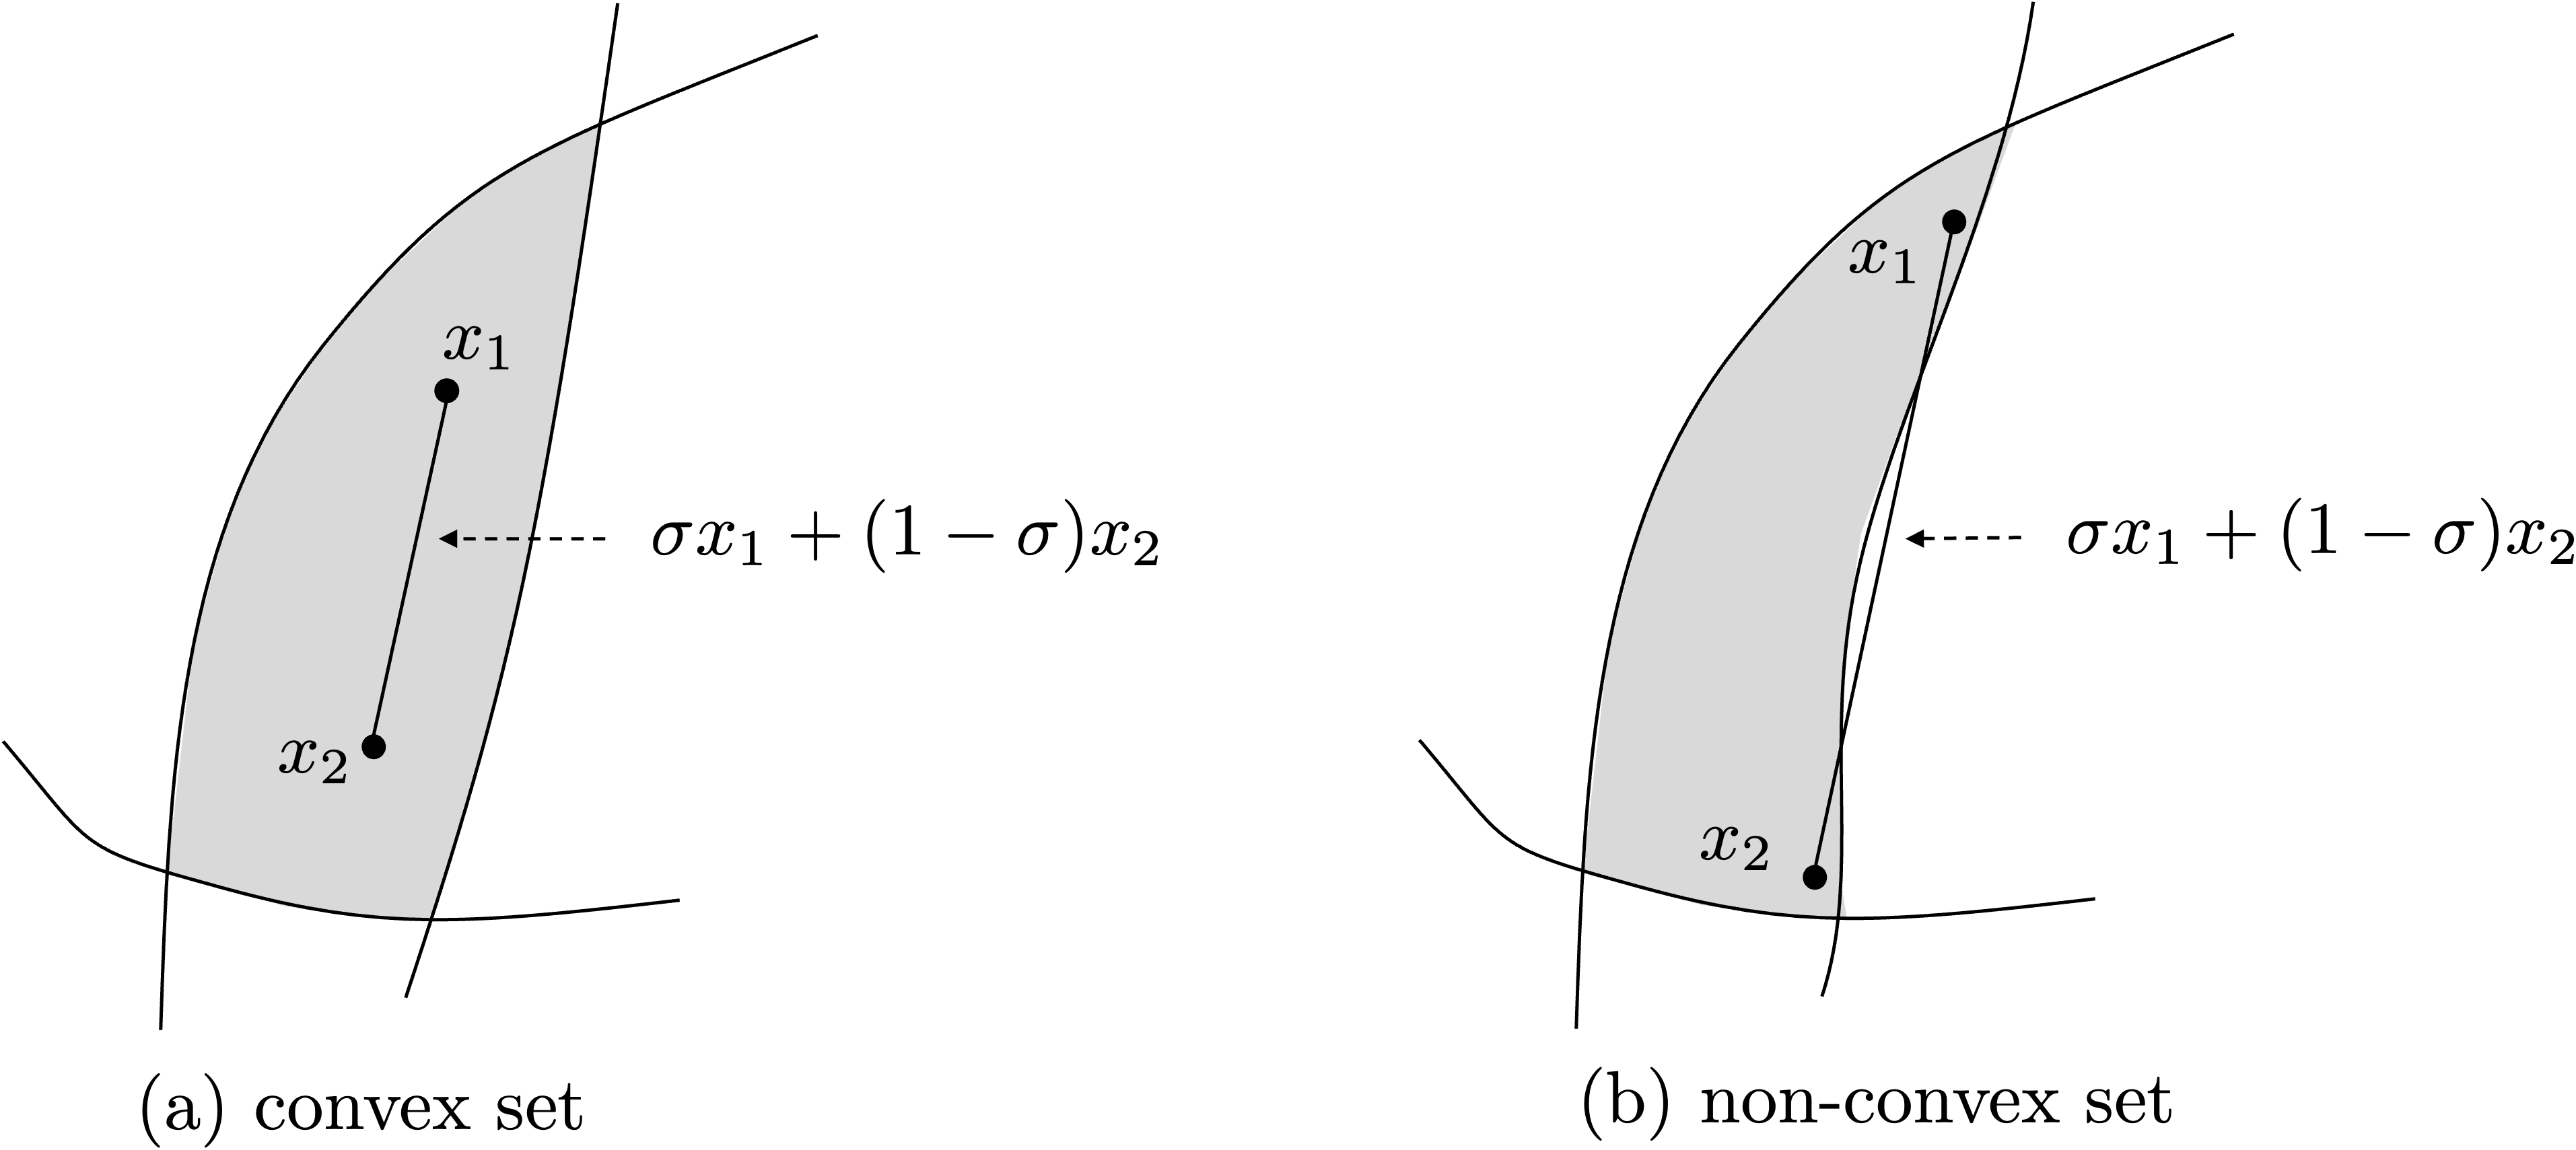
\includegraphics[width=0.9\textwidth]{figures/convex_set}
  \caption{(a) Convex set.  (b) Nonconvex set.}
  \label{fig:convex_set}
\end{figure}

The function $f:X\to \mathbb{R}$ is said to be convex if for every $x_1, x_2\in X$, and for every $\sigma\in[0, 1]$ we have
\[
f(\sigma x_1 + (1-\sigma)x_2) \leq \sigma f(x_1) + (1-\sigma)f(x_2).
\]
Note that $\sigma x_1 + (1-\sigma)x_2$ for $\sigma\in[0, 1]$ is the line connecting $x_1$ and $x_2$ in $X$, and that $\sigma f(x_1) + (1-\sigma)f(x_2)$ is the line connecting $f(x_1)$ and $f(x_2)$ in $\mathbb{R}$.  If $X=\mathbb{R}$, then $f$ is convex if the chord between $f(x_1)$ and $f(x_2)$ is greater than the function between $f(x_1)$ and $f(x_2)$ as shown in Figure~\ref{fig:convex_function}.
\begin{figure}[hbt]
  \centering
  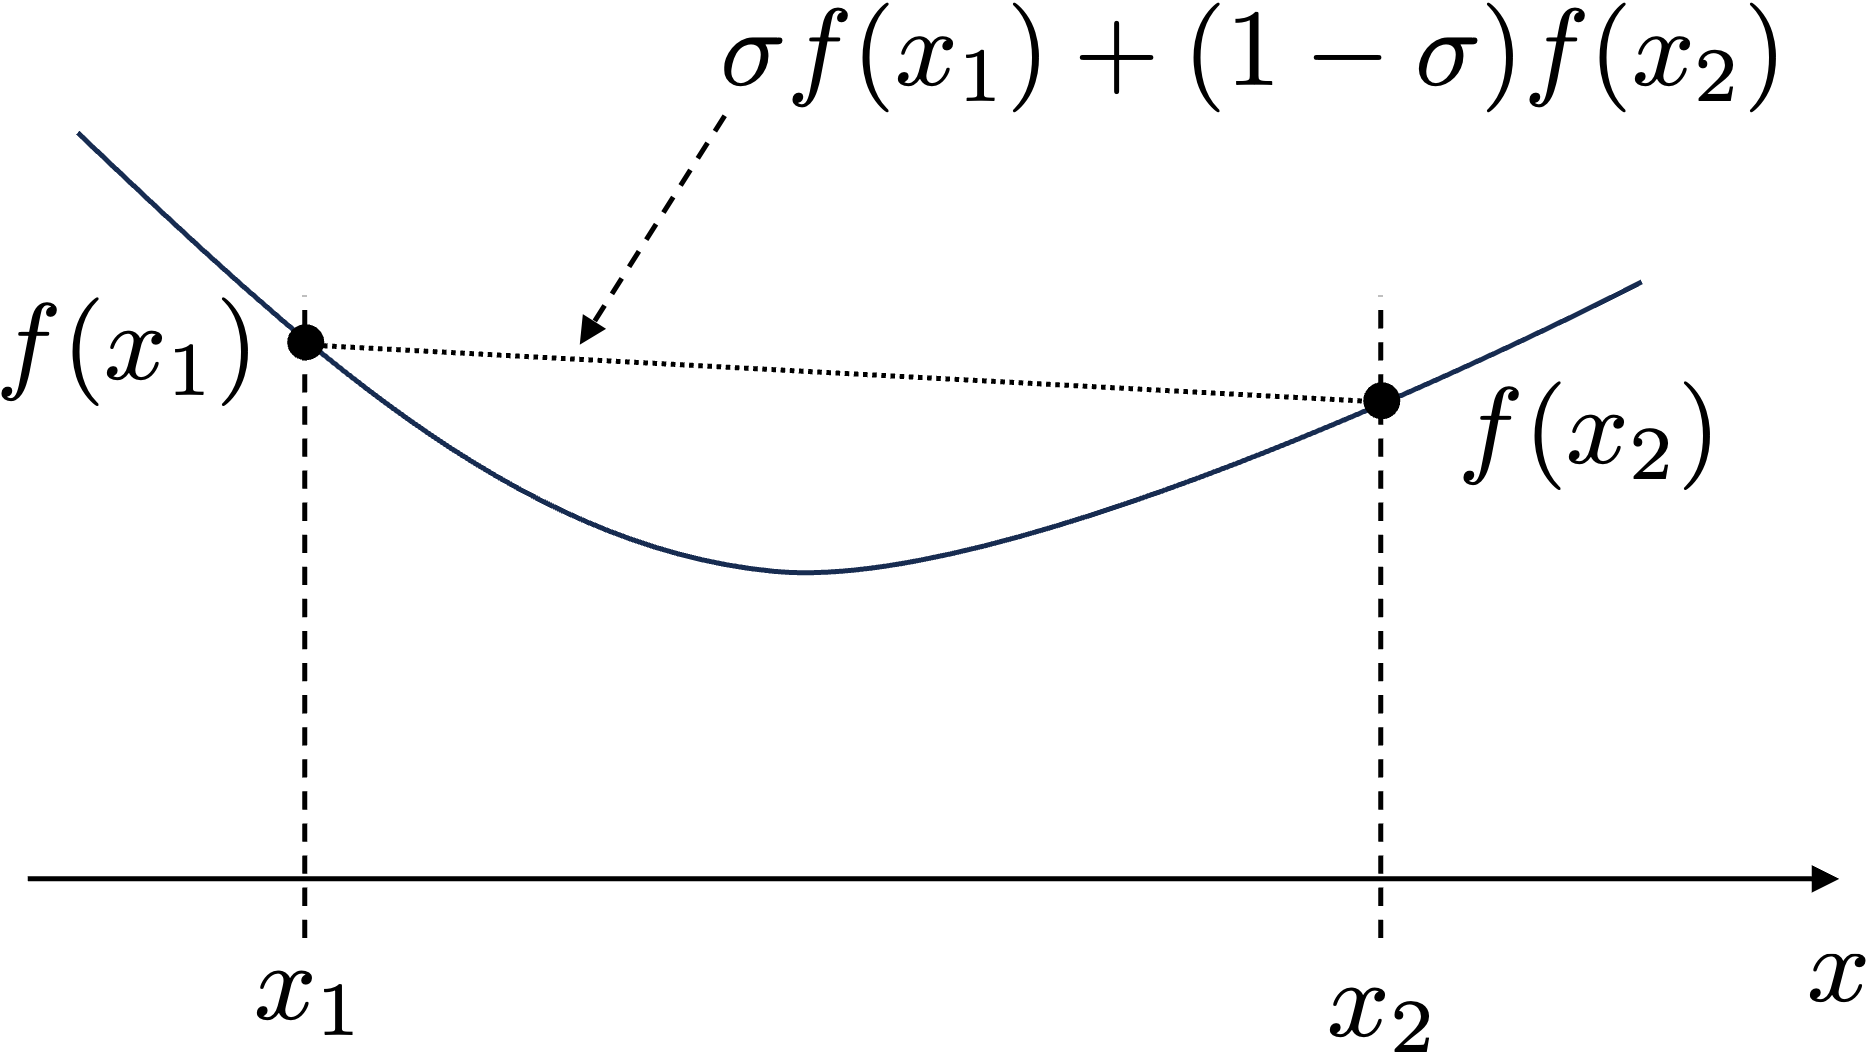
\includegraphics[width=0.5\textwidth]{figures/convex_function}
  \caption{Convex function}
  \label{fig:convex_function}
\end{figure}

The following properties are listed on Wikipedia (https://en.wikipedia.org/wiki/Convex\_function).
\begin{theorem}
The continuously differentiable function $f:\mathbb{R}^n \to \mathbb{R}^m$ is convex on $\Omega$ if and only if
\[
f(x_1) \geq f(x_2) + \nabla_x f(x_2) (x_1-x_2)
\]
for all $x_1, x_2\in\Omega\subseteq\mathbb{R}^n$.
\end{theorem}
\begin{theorem}
A twice differentiable function of several variables is convex on a convex set if and only if its Hessian matrix of second partial derivatives is positive semidefinite on the interior of the convex set.	
\end{theorem}
\begin{theorem}
The set of global minimisers of a convex function $f$, is a convex set, i.e.,
\[
\Omega = \{x: x=\arg\min f(\xi)\}
\]
is convex.
\end{theorem}
\begin{theorem}
Any local minimum of a convex function is also a global minimum.	
\end{theorem}

The following properties are also on Wikipedia~\url{https://en.wikipedia.org/wiki/Convex_function}.
\begin{theorem}
The following operations preserve convexity:
\begin{itemize}
	\item If $r$ is any real number then $r+f$ is convex if and only if $f$ is convex.
	\item Nonnegative weighted sums: If $w_1, \dots, w_n\geq 0$ and $f_1, \dots f_n$ are all convex, then $w_1f_1 + \dots w_n f_n$ is convex. This property extends to infinite sums, integrals and expected values as well (provided that they exist).
	\item Elementwise maximum: let $\{f_i\}_{i\in\mathcal{I}}$ be a collection of convex functions. Then $g(x) = \sup_{y\in\mathcal{I}}f_i(x)$ is convex.   The domain of $g(x)$ is the collection of points where the expression is finite. Important special cases:
		\begin{itemize}
			\item If $f_{1},\ldots ,f_{n}$ are convex functions then so is 
				\[ 
				g(x)=\max \left\{ f_{1}(x), \ldots, f_{n}(x) \right\}.
				\]
			\item Danskin's theorem: If $f(x,y)$ is convex in $x$ then $g(x)=\sup \nolimits _{y\in C}f(x,y)$ is convex in $x$ even if $C$ is not a convex set.
		\end{itemize}
	\item Composition: 
		\begin{itemize} 
			\item If $f$  and $g$ are convex functions and $g$ is non-decreasing over a univariate domain, then $h(x)=g(f(x))$ is convex. For example, if $f$ is convex, then so is $e^{f(x)}$ because $e^{x}$ is convex and monotonically increasing.
			\item If $f$ is concave and $g$ is convex and non-increasing over a univariate domain, then $h(x)=g(f(x))$ is convex.
			\item Convexity is invariant under affine maps: that is, if $f$ is convex with domain $D_{f}\subseteq \mathbb{R}^{m}$, then so is $g(x)=f(Ax+b)$, where $A\in \mathbb{R}^{m\times n}, b\in \mathbb{R}^{m}$ with domain $D_{g}\subseteq \mathbb{R}^{n}$.
		\end{itemize}
	\item Minimization: If $f(x,y)$ is convex in $(x,y)$ then $g(x)=\inf \nolimits _{y\in C}f(x,y)$ is convex in $x$, provided that $C$ is a convex set and that $g(x)\neq -\infty$.
	\item If $f$ is convex, then its perspective 
		\(
		g(x,t)=tf\left({\tfrac {x}{t}}\right)
		\) with domain 
		\[
		\left\{(x,t):{\tfrac {x}{t}}\in \operatorname {Dom} (f),t>0\right\}
		\]  is convex.
	\item Let $X$ be a vector space. $f:X\to \mathbb{R}$ is convex and satisfies $f(0)\leq 0$ if and only if $f(ax+by)\leq af(x)+bf(y)$ for any $x, y \in X$ and any non-negative real numbers $a,b$ that satisfy $a+b\leq 1$.	
 	
\end{itemize}

\end{theorem}

%---------------------------------------------------------------
\section{Newton's Method}

Given a function $J:\mathbb{R}^m\mapsto\mathbb{R}^n$, Newton's method can be used to find the zero of the function that is close to an initial starting point.  In other words, the objective is to find $x^\ast$ close to $x_0$ where $f(x^\ast)=0$.
The basic idea behind Newton's method is shown in Figure~\ref{fig:newtons_method} for $m=n=1$.
\begin{figure}[hbt]
  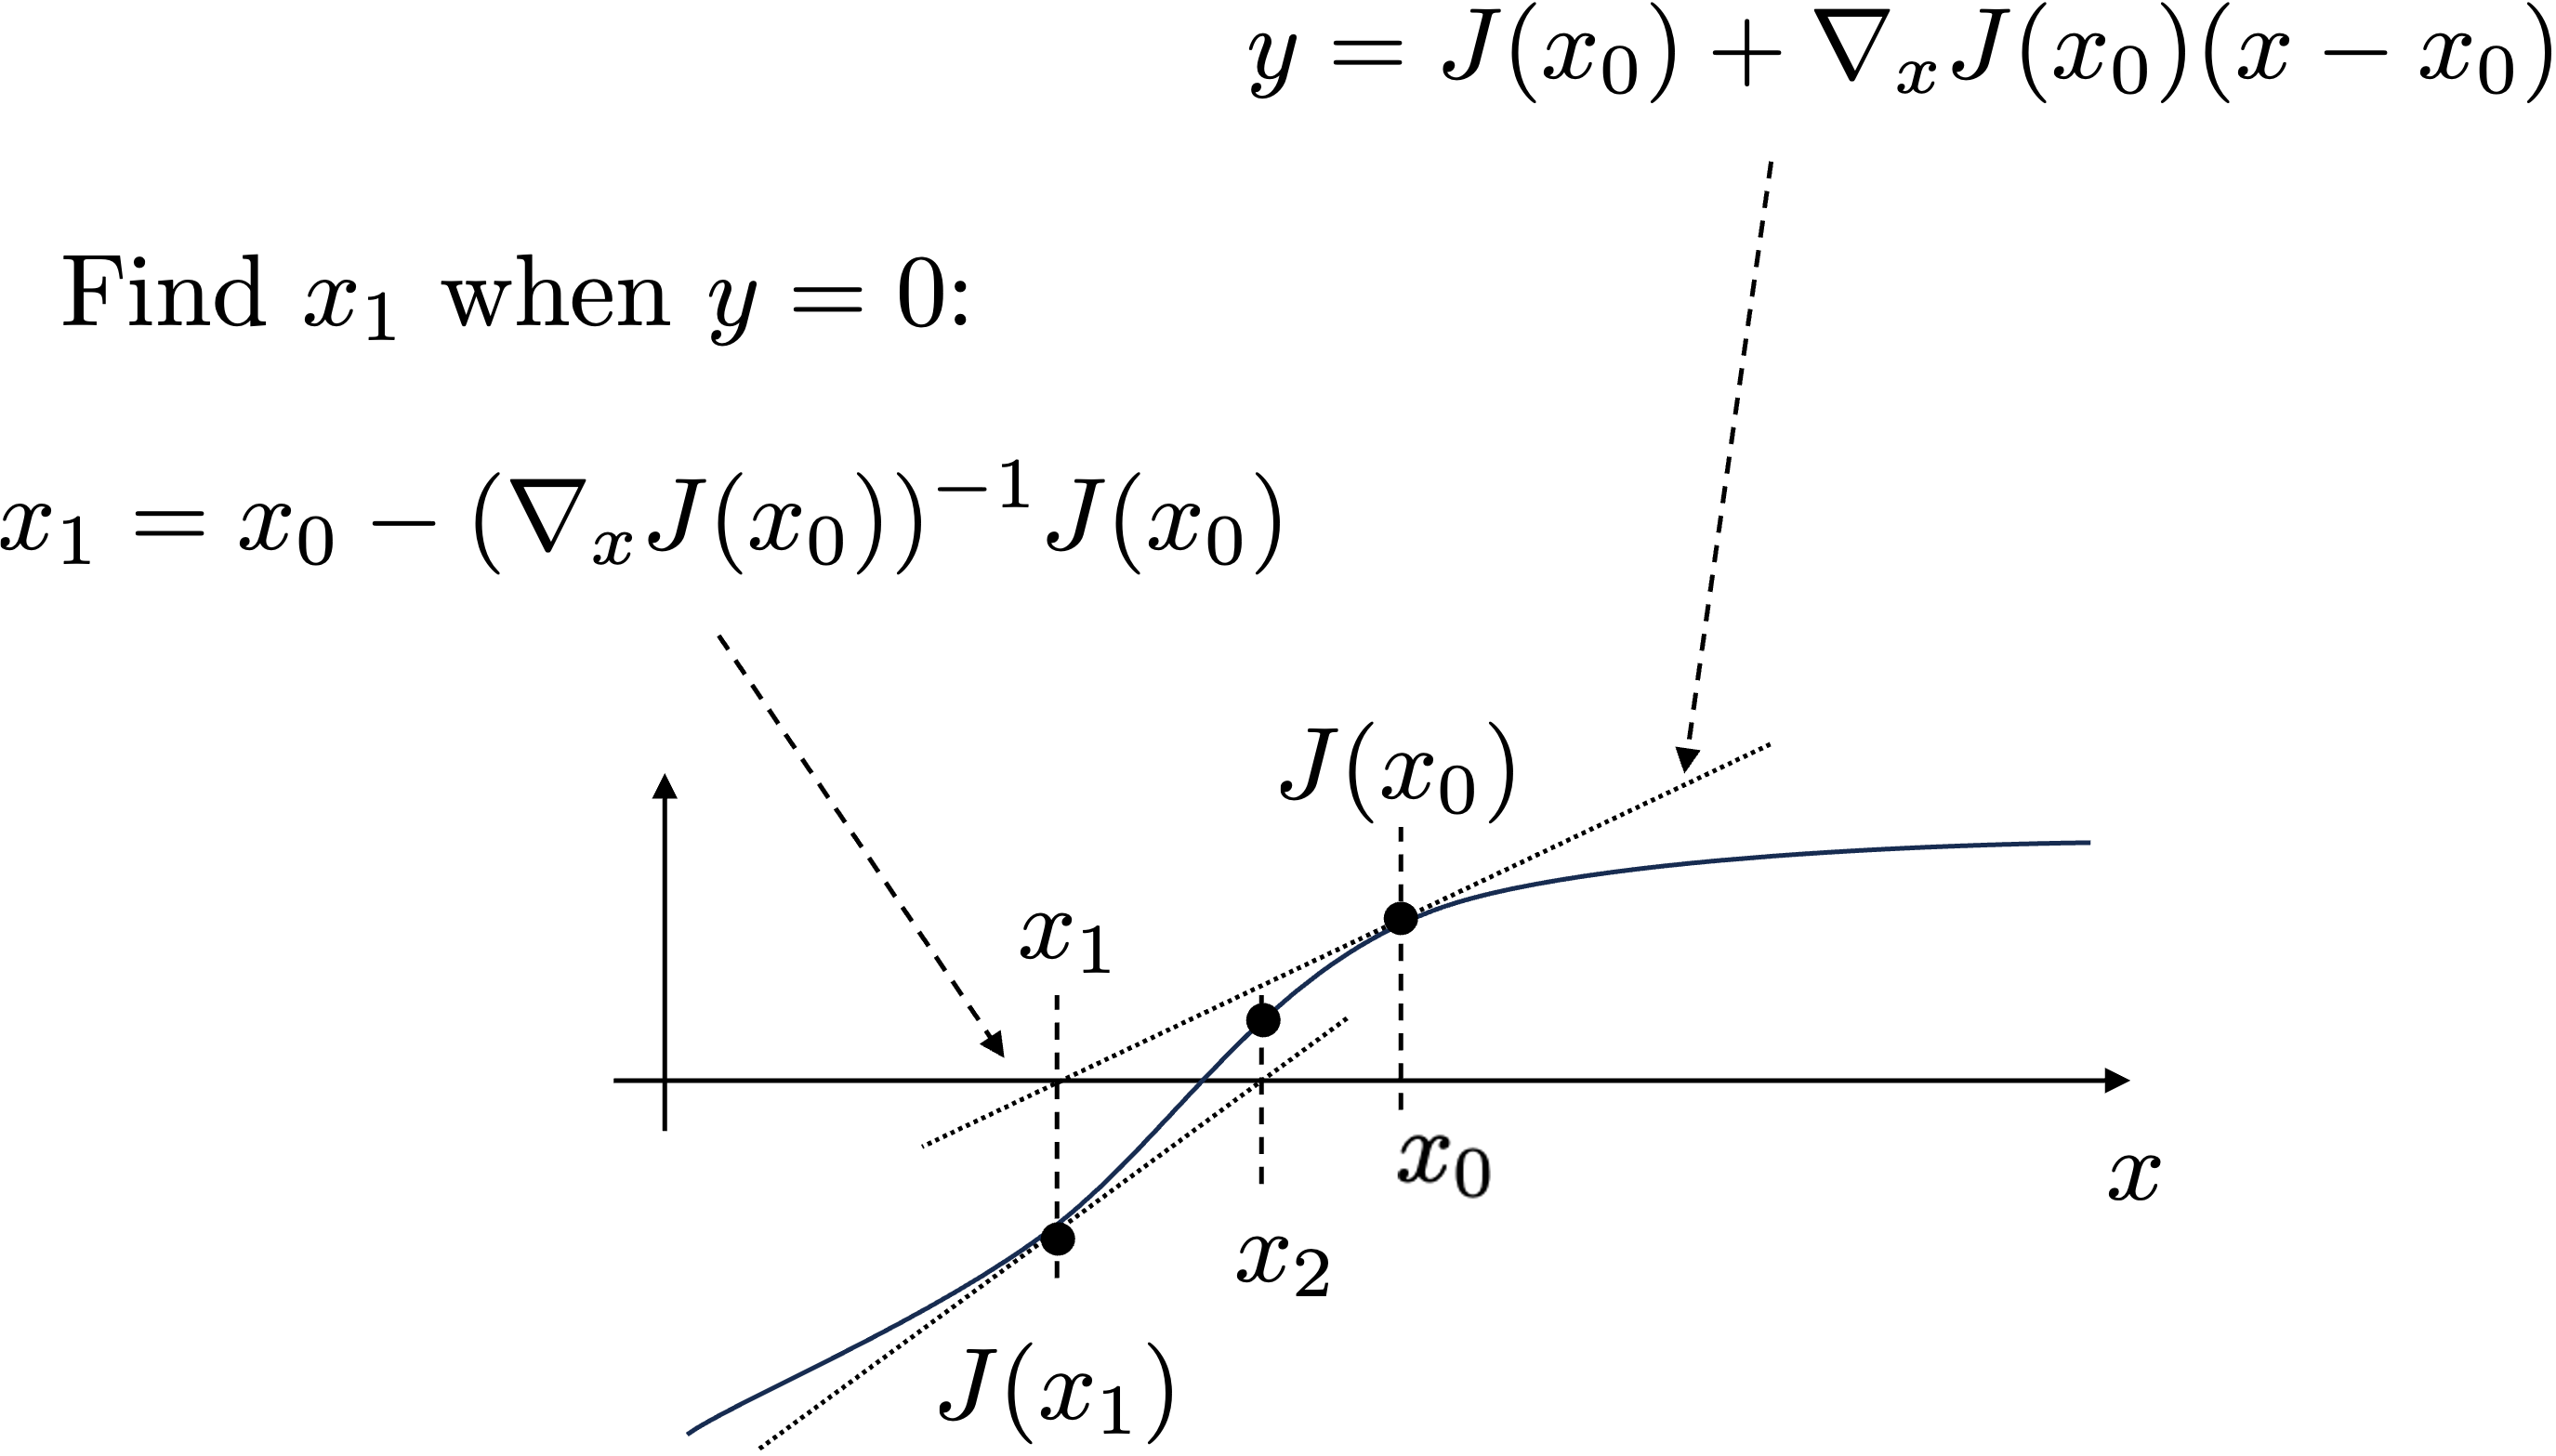
\includegraphics[width=0.9\textwidth]{figures/newtons_method}
  \caption{Newton's method}
  \label{fig:newtons_method}
\end{figure}
If $\nabla_x J(\hat{x})$ is the Jacobian of $J$ with respect to $x$ evaluated at $\hat{x}$, then the linear approximation to $J$ at $x_0$ is given by
\[
y = J(x_0) + \left(\nabla_x J(x_0)\right) (x-x_0).
\]
As shown in Figure~\ref{fig:newtons_method}, if we let $x_1$ be the location where the linear approximation is zero, then
\[
x_1 = x_0 - \left(\nabla_x J(x_0)\right)^{-1} J(x_0).
\]
This process can then be iterated to find the zero of the function using the iteration
\[
x_k = x_{k-1} - \left(\nabla_x J(x_{k-1})\right)^{-1} J(x_{k-1}).
\]
It is well known that $x_k\to x^\ast$ quadratically if $x_0\in B_{\epsilon}(x^\ast)$ implies that
\begin{itemize}
\item 	$\nabla_x J(x)$ is non-zero on $B_{\epsilon}(x^\ast)$, 
\item $\nabla_x^2 J(x)$ is continuous on $B_{\epsilon}(x^\ast)$,
\item $\frac{\sup_{\hat{x}\in B_{\epsilon}(x^\ast)}
       \norm{\nabla_x^2 J(\hat{x})}}
       {\inf_{\hat{x}\in B_{\epsilon}(x^\ast)}\norm{\nabla_x(J(\hat{x})}} < \frac{2}{\epsilon}
       $
\end{itemize}

Alternatively, Newton's method can be written in two steps:
\begin{align*}
&\text{\bf Step 1,~solve for feasible direction $\mathbf{p}$:~} \qquad	\left(\nabla_x J(x_{k-1})\right) \mathbf{p} = J(x_{k-1}) \\
&\text{\bf Step 2, update $x$ along feasible direction:~} \qquad x_k = x_{k-1} - \mathbf{p},
\end{align*}
where the equation
\[
\left(\nabla_x J(x_{k-1})\right) \mathbf{p} = J(x_{k-1})
\]
can be solved efficiently by computing the QR decomposition of $\nabla_x J(x_{k-1})$:
\[
QR = \nabla_x J(x_{k-1})
\]
where $Q$ is unitary and $R$ is upper triangular.  The vector $\mathbf{p}$ can be found by back-substitution of the equation
\[
R\mathbf{p} = Q^\top J(x_{k-1}).
\]


%---------------------------------------------------------------
\section{Interior Point Methods}

The discussion in this section is adapted from \url{https://en.wikipedia.org/wiki/Interior-point_method}.

Consider the inequality constrained optimization problem
			\begin{mini*}|s|
				{}{f(x)}{}{}
				\addConstraint{\gbf(x) \geq 0}
			\end{mini*}
			where $\gbf(x) \geq 0$ means that
			\[
				\begin{pmatrix}
			    	g_1(x)\\
			    	\vdots\\
			    	g_q(x)
			  	\end{pmatrix} 
			  	\geq \begin{pmatrix} 
		 				0 \\ \vdots \\ 0
					 \end{pmatrix}
			\]
			i.e., element-wise,
	and assume that $f:\mathbb{R}^n\to\mathbb{R}$ is a convex function, and that the constraint region
	\[
		\Omega = \bigcap_{i=1}^q \{x\in\mathbb{R}^n | g_i(x) \geq 0\}
	\]
	is convex, and suppose that there is an initial guess in the interior of $\Omega$, i.e., $x_0\in\Omega$. Since $\Omega$ is convex, if $x_0$ is interior to $\Omega$, then every direction is a feasible direction, and a small enough step will remain in $\Omega$.  The idea is to construct barrier functions that keep the next guess inside $\Omega$.  The convexity of $f$ and $\Omega$ ensures that gradient descent {\bf inside} $\Omega$ will find a global solution.
	
	Construct the logarithmic barrier function
	\[
	B(x, \mu) \triangleq f(x) - \mu\sum_{i=1}^q \log(g_i(x)).
	\]
	Note that close to the boundary where $0<g_i(x)=\epsilon$ that as $\epsilon\to 0$, that $B(x,\mu)\to\infty$, with the cost being infinite on the boundary for any $\mu\neq 0$. 
	Also note that as $\mu\to 0$, that $B(x,\mu)\to f(x)$ except on the boundary $\partial\Omega$, where $B(x,\mu)=\infty$.  
	
	The idea is therefore to solve the unconstrained optimization problem 
		\begin{mini*}|s|
				{x\in\Omega}{B(x,\mu)}{}{}
		\end{mini*}
	using standard methods, 	and then to decrease $\mu\to 0$ until convergence happens either inside $\Omega$ or to a point in the boundary $\partial\Omega$.
	
	
	Taking the gradient with respect to $x$ gives
	\[
	\nabla_x B(x, \mu) = \nabla_x f(x) - \mu\sum_{i=1}^q \frac{\nabla_x g_i(x)}{g_i(x)}.
	\]	
	Introduce the Lagrange multipliers (actually, the dependence on $x$, means that they are not true Lagrange multipliers)
	\[
	\lambda_i(x) \triangleq \frac{\mu}{g_i(x)}
	\]
	then for a fixed $\mu$, the necessary conditions become
	\begin{align*}
	H(x_\mu, \boldsymbol{\lambda}_{\mu}) \triangleq 
		\begin{bmatrix}
 			\nabla_x f(x_\mu) - \nabla_x \mathbf{g}(x_\mu) \boldsymbol{\lambda}_\mu \\
 			\mu I - \text{diag}(\mathbf{g}(x_\mu))\boldsymbol{\lambda}_{\mu}
 		\end{bmatrix} = 0.
	\end{align*}
	
	Using Newton's method to find the zeros, we first compute the update 
	\begin{align*}
	& \nabla H \mathbf{p} = H \\
	\implies & \begin{bmatrix}
					\nabla_x^2 f(x_\mu) - \sum_{i=1}^q \nabla_x^2 g_i(x_\mu) \lambda_i & -\nabla_x \mathbf{g}(x_\mu) \\
					-\nabla_x\left(\text{diag}(\mathbf{g}(x_\mu))\boldsymbol{\lambda}_{\mu}\right) & -\text{diag}(\mathbf{g}(x_\mu))
               \end{bmatrix}
               \begin{pmatrix} \mathbf{p}_x \\ \mathbf{p}_\lambda \end{pmatrix}	
               = \begin{bmatrix}
 					\nabla_x f(x_\mu) - \nabla_x \mathbf{g}(x_\mu) \boldsymbol{\lambda}_\mu \\
 					\mu I - \text{diag}(\mathbf{g}(x_\mu))\boldsymbol{\lambda}_{\mu}
 				\end{bmatrix}
	\end{align*}
	using QR factorization, and then update $(x_\mu, \lambda_\mu)$ as
\[
	\begin{pmatrix} x_{\mu, k} \\ \boldsymbol{\lambda}_{\mu, k} \end{pmatrix} 
	= \begin{pmatrix} x_{\mu, k-1} \\ \boldsymbol{\lambda}_{\mu, k-1} \end{pmatrix} - \alpha \begin{pmatrix} \mathbf{p}_x \\ \mathbf{p}_{\lambda} \end{pmatrix}
\]
where $\alpha$ is nominally equal to 1, but may be decreased to ensure that each $\lambda_i\geq 0$.

This process is carried to convergence.  The parameter $\mu$ is then decreased and the process is repeated using the converged values as the initial conditions for the problem with a new $\mu$.  This process is continued until $x_\mu$ and $\boldsymbol{\lambda}_{\mu}$ converges for iterations in $\mu$.
	
	
	

	










% Bibliography
\bibliography{/Users/beard/Dropbox/papers/bib/library.bib}
\bibliographystyle{IEEEtran}

\end{document}